\chapter{\PrintfSeveralArgumentsSectionName}

\RU{Попробуем теперь немного расширить пример \IT{\HelloWorldSectionName}~(\ref{sec:helloworld}),
написав в теле функции \main:}
\EN{Now let's extend the \IT{\HelloWorldSectionName}~(\ref{sec:helloworld}) example, replacing \printf in
the \main function body by this:}

\lstinputlisting[label=hw_c]{patterns/03_printf/1.c}

% sections
\sectionold{x86}

% subsections:
\subsection{x86: \RU{3 аргумента}\EN{3 arguments}}

\subsubsection{MSVC}

\RU{Компилируем при помощи MSVC 2010 Express, и в итоге получим:}
\EN{When we compile it with MSVC 2010 Express we get:}

\begin{lstlisting}
$SG3830	DB	'a=%d; b=%d; c=%d', 00H

...

	push	3
	push	2
	push	1
	push	OFFSET $SG3830
	call	_printf
	add	esp, 16					; 00000010H
\end{lstlisting}

\RU{Все почти то же, за исключением того, что теперь видно, что аргументы для \printf заталкиваются в стек в обратном порядке: самый первый аргумент заталкивается последним.}
\EN{Almost the same, but now we can see the \printf arguments are pushed onto the stack in reverse order. The first argument is pushed last.}

\RU{Кстати, вспомним что переменные типа \Tint в 32-битной системе, как известно, имеет ширину 32 бита, это 4 байта}
\EN{By the way, variables of \Tint type in 32-bit environment have 32-bit width, that is 4 bytes}.

\RU{Итак, у нас всего 4 аргумента. $4*4 = 16$ ~--- именно 16 байт занимают в стеке указатель на строку плюс еще 3 числа типа \Tint.}
\EN{So, we have 4 arguments here. $4*4 = 16$~---they occupy exactly 16 bytes in the stack: a 32-bit pointer to a string and 3 numbers of type \Tint.}

\index{x86!\Instructions!ADD}
\index{x86!\Registers!ESP}
\index{cdecl}
\RU{Когда при помощи инструкции \TT{ADD ESP, X} корректируется \glslink{stack pointer}{указатель стека} \ESP 
после вызова какой-либо функции, зачастую можно сделать вывод о том, сколько аргументов 
у вызываемой функции было, разделив X на 4.}
\EN{When the \gls{stack pointer} (\ESP register) has changed back by the \TT{ADD ESP, X}
instruction after a function 
call, often, the number of function arguments could be deduced by simply dividing X by 4.}

\RU{Конечно, это относится только к cdecl-методу передачи аргументов через стек, 
и только для 32-битной среды.}
\EN{Of course, this is specific to the \IT{cdecl} calling convention, 
and only for 32-bit environment.}

\ifx\LITE\undefined
\RU{См. также в соответствующем разделе о способах передачи аргументов через стек}
\EN{See also the calling conventions section}~(\myref{sec:callingconventions}).
\fi

\RU{Иногда бывает так, что подряд идут несколько вызовов разных функций, 
но стек корректируется только один раз, после последнего вызова:}
\EN{In certain cases where several functions return right after one another, the compiler could merge multiple \TT{``ADD ESP, X''} instructions into one, after the last call:}

\begin{lstlisting}
push a1
push a2
call ...
...
push a1
call ...
...
push a1
push a2
push a3
call ...
add esp, 24
\end{lstlisting}

\RU{Вот пример из реальной жизни:}
\EN{Here is a real-world example:}

\lstinputlisting[caption=x86]{patterns/03_printf/x86/add_example.lst.\LANG}

\ifdefined\IncludeOlly
\clearpage
\subsubsection{MSVC \AndENRU \olly}
\index{\olly}

\RU{Попробуем этот же пример в}\EN{Now let's try to load this example in} \olly.
\RU{Это один из наиболее популярных win32-отладчиков user-режима}\EN{It is one of the most 
popular user-land win32 debuggers}.
\RU{Мы можем компилировать наш пример в}\EN{We can compile our example in} MSVC 2012 
\RU{с опцией}\EN{with} \TT{/MD} \RU{что означает, линковать с библиотекой}\EN{option, which means to link 
with} \TT{MSVCR*.DLL},
\RU{чтобы импортируемые функции были хорошо видны в отладчике.}
\EN{so we can see the imported functions clearly in the debugger.}

\RU{Затем загружаем исполняемый файл в}\EN{Then load the executable in} \olly.
\RU{Самый первый брякпойнт в}\EN{The very first breakpoint is in} \TT{ntdll.dll}, \RU{нажмите}\EN{press} 
F9 (\RU{запустить}\EN{run}).
\RU{Второй брякпойнт в}\EN{The second breakpoint is in} \ac{CRT}-\RU{коде}\EN{code}.
\RU{Теперь мы должны найти функцию}\EN{Now we have to find the} \main\EN{ function}.

\RU{Найдите этот код скроллируя окно кода до самого верха (MSVC располагает функцию \main в самом начале
секции кода)}\EN{Find this code by scrolling the code to the very top (MSVC allocates the \main function at
the very beginning of the code section)}: 

\begin{figure}[H]
\centering
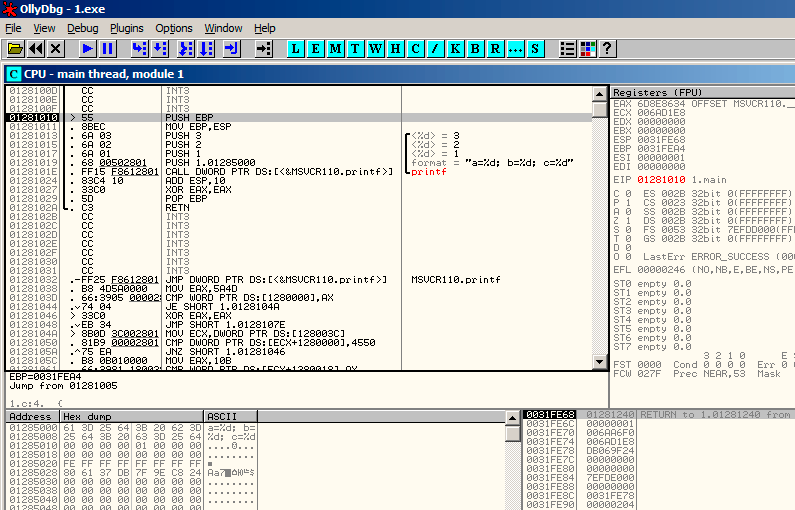
\includegraphics[scale=\FigScale]{patterns/03_printf/x86/olly3_1.png}
\caption{\olly: \RU{самое начало функции}\EN{the very start of the} \main\EN{ function}}
\label{fig:printf3_olly_1}
\end{figure}

\RU{Кликните на инструкции}\EN{Click on the} \TT{PUSH EBP}\RU{, нажмите}\EN{ instruction, press} F2 
(\RU{установка брякпойнта}\EN{set breakpoint}) \RU{и нажмите}\EN{and press} F9 (\RU{запустить}\EN{run}).
\RU{Нам нужно произвести все эти манипуляции, чтобы пропустить \ac{CRT}-код, потому что нам он пока
не интересен}\EN{We need to perform these actions in order to skip \ac{CRT}-code, because we aren't really
interested in it yet}.

\clearpage
\RU{Нажмите}\EN{Press} F8 (\stepover) 6 \RU{раз, т.е., пропустить
6 инструкций}\EN{times, i.e., skip 6 instructions}:

\begin{figure}[H]
\centering
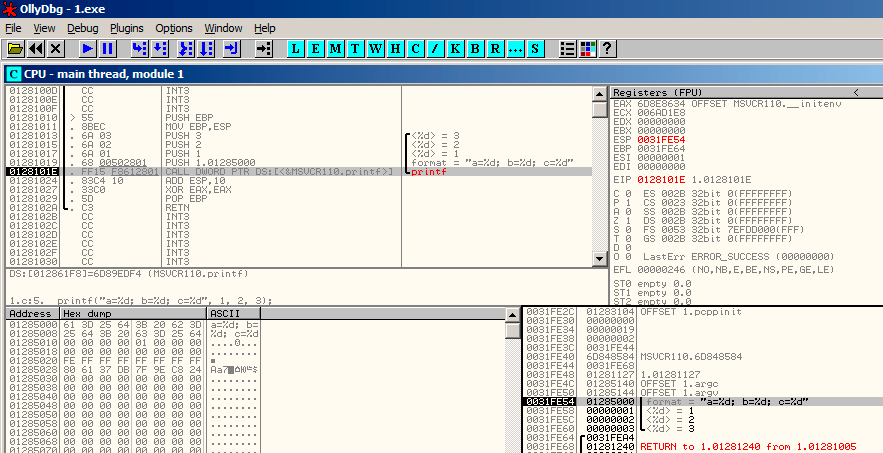
\includegraphics[scale=\FigScale]{patterns/03_printf/x86/olly3_2.png}
\caption{\olly: \RU{перед исполнением}\EN{before} \printf\EN{ execution}}
\label{fig:printf3_olly_2}
\end{figure}

\RU{Теперь}\EN{Now the} \ac{PC} \RU{указывает на инструкцию}\EN{points to the}
\TT{CALL printf}\EN{ instruction}.
\olly, \RU{как и другие отладчики, подсвечивает регистры со значениями, которые изменились}
\EN{like other debuggers, highlights the value of the registers which were changed}.
\RU{Так что, каждый раз, когда мы нажимаем}\EN{So each time you press F8}, \EIP 
\RU{изменяется и его значение подсвечивается красным}\EN{ changes and its value is displayed in red}.
\ESP \RU{также меняется, потому что значения заталкиваются в стек}\EN{changes as well, 
because the arguments values are pushed into the stack}.\\
\\
\RU{Где находятся эти значения в стеке}\EN{Where are the values in the stack}?
\RU{Посмотрите на правое/нижнее окно в отладчике}\EN{Take a look at the right/bottom debugger window}:

\begin{figure}[H]
\centering
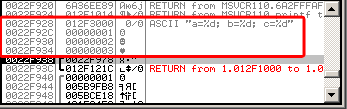
\includegraphics[scale=\NormalScale]{patterns/03_printf/x86/olly3_stack.png}
\caption{\olly: \RU{стек, после того как значения там сохранены}\EN{stack after the argument values have been pushed}
(\RU{я сделал здесь округлую красную пометку в графическом редакторе}\EN{The red rectangular border was added by me in a graphics editor})}
\end{figure}

\RU{Так что здесь видно 3 столбца: адрес в стеке, значение в стеке и еще дополнительный комментарий
от \olly}\EN{We can see 3 columns there: address in the stack, 
value in the stack and some additional \olly comments}. 
\olly \RU{понимает}\EN{understands} \printf\RU{-строки}\EN{-like strings}, 
\RU{так что он показывает здесь и строку и 3 значения \IT{привязанных} к ней}\EN{so it reports the 
string here and the 3 values \IT{attached} to it}.

\RU{Можно кликнуть правой кнопкой мыши на строке формата, кликнуть на ``Follow in dump''
и строка формата появится в окне слева внизу, где всегда виден какой-либо участок памяти}
\EN{It is possible to right-click on the format string, click on ``Follow in dump'',
and the format string will appear in the debugger left-bottom window, which always displays some part of the memory}.
\RU{Эти значения в памяти можно редактировать}\EN{These memory values can be edited}.
\RU{Можно изменить саму строку формата, и тогда результат работы нашего примера будет другой}
\EN{It is possible to change the format string, in which case the result of our example would be different}.
\RU{В данном случае, пользы от этого немного, но для упражнения это полезно,
чтобы начать чувствовать как тут всё работает}\EN{It is not very useful in this particular case, but it could be good as an exercise so you start building a feel of how everything works here}.

\clearpage
\RU{Нажмите}\EN{Press} F8 (\stepover).

\RU{В консоли мы видим вывод}\EN{We see the following output in the console}:

\begin{figure}[H]
\centering
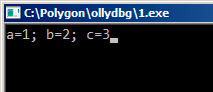
\includegraphics[scale=\NormalScale]{patterns/03_printf/x86/olly3_console.png}
\caption{\RU{Ф-ция }\printf \RU{исполнилась}\EN{function executed}}
\end{figure}

\RU{Посмотрим, как изменились регистры и состояние стека}\EN{Let's see how the registers and stack state 
have changed}: 

\begin{figure}[H]
\centering
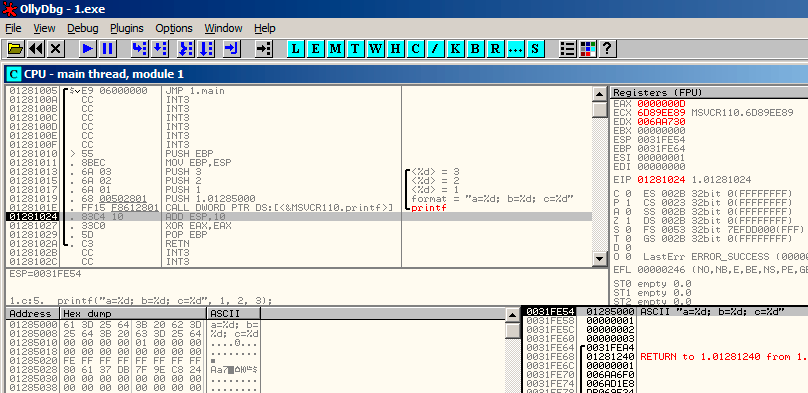
\includegraphics[scale=\FigScale]{patterns/03_printf/x86/olly3_3.png}
\caption{\olly: \RU{после исполнения}\EN{after} \printf\EN{ execution}}
\label{fig:printf3_olly_3}
\end{figure}

\RU{Регистр }\EN{Register }\EAX \RU{теперь содержит}\EN{now contains} \TT{0xD} (13).
\RU{Всё верно: \printf возвращает количество выведенных символов.
Значение \EIP изменилось: действительно, теперь здесь адрес инструкции после 
\TT{CALL printf}.}
\EN{That is correct, since \printf returns the number of characters printed. 
The value of \EIP has changed: indeed, now it contains the address of the instruction coming after 
\TT{CALL printf}.}
\RU{Значения регистров }\ECX \AndENRU \EDX \RU{также изменились}\EN{values have changed as well}.
\RU{Очевидно, внутренности функции \printf используют их для каких-то своих нужд}\EN{Apparently, the 
\printf function's hidden machinery used them for its own needs}.

\RU{Очень важный момент в том, что значение \ESP не изменилось. И аргументы-значения в стеке также!}
\EN{A very important fact is that neither the \ESP value, nor the stack state have been changed!}
\RU{Мы ясно видим здесь и строку формата и соответствующие ей 3 значения, они все еще здесь.}
\EN{We clearly see that the format string and corresponding 3 values are still there.}
\RU{Действительно, по соглашению вызовов \IT{cdecl}, вызываемая функция не возвращает \ESP назад.}
\EN{This is indeed the \IT{cdecl} calling convention behaviour: \gls{callee} does not return \ESP back to its previous value.}
\RU{Это должна делать вызывающая функция}\EN{The \gls{caller} is responsible to do so}.

\clearpage
\RU{Нажмите}\EN{Press} F8 \RU{снова, чтобы исполнилась инструкция}\EN{again to execute} 
\TT{ADD ESP, 10}\EN{ instruction}:

\begin{figure}[H]
\centering
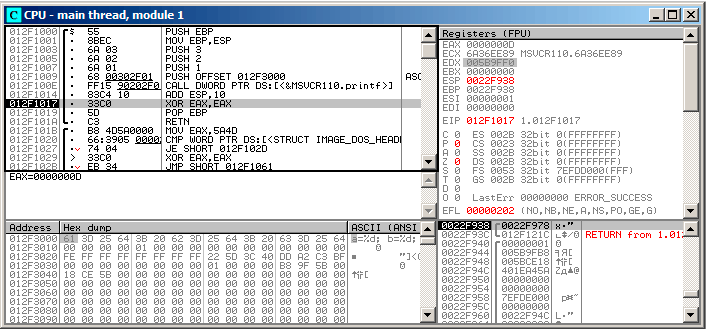
\includegraphics[scale=\FigScale]{patterns/03_printf/x86/olly3_4.png}
\caption{\olly: \RU{после исполнения инструкции}\EN{after} \TT{ADD ESP, 10}\EN{ instruction execution}}
\label{fig:printf3_olly_4}
\end{figure}

\ESP \RU{изменился, но значения все еще в стеке}\EN{has changed, but the values are still in the stack}!
\RU{Конечно, никому не нужно заполнять эти значения нулями или что-то в этом роде}\EN{Yes, 
of course; no one needs to set these values to zeroes or something like that}
\RU{Потому что всё что выше указателя стека.}\EN{because everything above the stack pointer} (\ac{SP}) 
\RU{это}\EN{is} \IT{\RU{шум}\EN{noise}} \OrENRU \IT{\garbage{}}, \RU{это всё не имеет
особой ценности}\EN{and has no meaning at all}.
\RU{Было бы очень затратно по времени очищать ненужные элементы стека, к тому же, никому это и не 
нужно}\EN{It would be time consuming to clear the unused stack entries anyway, and no one really needs to}.

\fi

\ifdefined\IncludeGCC
\subsubsection{GCC}

\RU{Скомпилируем то же самое в Linux при помощи GCC 4.4.1 и посмотрим в \IDA что вышло:}
\EN{Now let's compile the same program in Linux using GCC 4.4.1 and take a look at what we have got in \IDA:}

\begin{lstlisting}
main            proc near

var_10          = dword ptr -10h
var_C           = dword ptr -0Ch
var_8           = dword ptr -8
var_4           = dword ptr -4

                push    ebp
                mov     ebp, esp
                and     esp, 0FFFFFFF0h
                sub     esp, 10h
                mov     eax, offset aADBDCD ; "a=%d; b=%d; c=%d"
                mov     [esp+10h+var_4], 3
                mov     [esp+10h+var_8], 2
                mov     [esp+10h+var_C], 1
                mov     [esp+10h+var_10], eax
                call    _printf
                mov     eax, 0
                leave
                retn
main            endp
\end{lstlisting}

\RU{Можно сказать, что этот короткий код, созданный GCC, отличается от кода MSVC только способом помещения 
значений в стек.
Здесь GCC снова работает со стеком напрямую без \PUSH/\POP.}
\EN{Its noticeable that the difference between the MSVC code and the GCC code is only in the way the arguments are stored on the stack.
Here the GCC is working directly with the stack without the use of \PUSH/\POP.}

\ifdefined\IncludeGDB
\subsubsection{GCC \AndENRU GDB}
\index{GDB}

\RU{Попробуем также этот пример и в \ac{GDB} в Linux}\EN{Let's try this example also in \ac{GDB} in Linux}.

\TT{-g} \RU{означает генерировать отладочную информацию в выходном исполняемом файле}\EN{option instructs the compiler to include debug information in the executable file}.

\begin{lstlisting}
$ gcc 1.c -g -o 1
\end{lstlisting}

\begin{lstlisting}
$ gdb 1
GNU gdb (GDB) 7.6.1-ubuntu
Copyright (C) 2013 Free Software Foundation, Inc.
License GPLv3+: GNU GPL version 3 or later <http://gnu.org/licenses/gpl.html>
This is free software: you are free to change and redistribute it.
There is NO WARRANTY, to the extent permitted by law.  Type "show copying"
and "show warranty" for details.
This GDB was configured as "i686-linux-gnu".
For bug reporting instructions, please see:
<http://www.gnu.org/software/gdb/bugs/>...
Reading symbols from /home/dennis/polygon/1...done.
\end{lstlisting}

\begin{lstlisting}[caption=\RU{установим брякпойнт на}\EN{let's set breakpoint on} \printf]
(gdb) b printf
Breakpoint 1 at 0x80482f0
\end{lstlisting}

\RU{Запукаем}\EN{Run}.
\RU{Здесь у нас нет исходного кода функции}\EN{We don't have the} \printf 
\RU{так что \ac{GDB} не может показать его исходный код, но могла бы}\EN{function source code here, 
so \ac{GDB} can't show it, but may do so}.

\begin{lstlisting}
(gdb) run
Starting program: /home/dennis/polygon/1 

Breakpoint 1, __printf (format=0x80484f0 "a=%d; b=%d; c=%d") at printf.c:29
29	printf.c: No such file or directory.
\end{lstlisting}

\RU{Выдать 10 элементов стека. Левый столбец --- это адрес в стеке.}
\EN{Print 10 stack elements. The most left column contains addresses on the stack.}

\begin{lstlisting}
(gdb) x/10w $esp
0xbffff11c:	0x0804844a	0x080484f0	0x00000001	0x00000002
0xbffff12c:	0x00000003	0x08048460	0x00000000	0x00000000
0xbffff13c:	0xb7e29905	0x00000001
\end{lstlisting}

\RU{Самый первый элемент это}\EN{The very first element is the} \ac{RA} (\TT{0x0804844a}).
\RU{Мы можем удостовериться в этом, дизассемблируя память по этому адресу}\EN{We can verify this by disassembling the memory at this address}:

\begin{lstlisting}
(gdb) x/5i 0x0804844a
   0x804844a <main+45>:	mov    $0x0,%eax
   0x804844f <main+50>:	leave  
   0x8048450 <main+51>:	ret    
   0x8048451:	xchg   %ax,%ax
   0x8048453:	xchg   %ax,%ax
\end{lstlisting}

\RU{Две инструкции}\EN{The two} \TT{XCHG} 
\RU{это, вероятно, какой-то случайный мусор, который мы пока что можем игнорировать}
\EN{instructions are probably random garbage, which we can ignore for now}.

\RU{Второй элемент}\EN{The second element} (\TT{0x080484f0}) \RU{это адрес
строки формата}\EN{is the format string address}:

\begin{lstlisting}
(gdb) x/s 0x080484f0
0x80484f0:	"a=%d; b=%d; c=%d"
\end{lstlisting}

\RU{Остальные 3 элемента}\EN{Next 3 elements} (1, 2, 3) \RU{это аргументы функции}\EN{are the} 
\printf\EN{ arguments}.
\RU{Остальные элементы это может быть и мусор в стеке, но могут быть и значения
от других функций, их локальные переменные, \etc{}.}
\EN{The rest of the elements could be just ``garbage'' on the stack,
but could also be values from other functions, their local variables, \etc{}.}
\RU{Пока что мы можем игнорировать их}\EN{We can ignore them for now}.

\RU{Исполняем}\EN{Run} ``finish''. 
\RU{Это значит, исполнять все инструкции до самого конца функции}\EN{The command instructs GDB to ``execute all instructions until the end of the function''}. 
\RU{Здесь это означает: исполнять до завершения}\EN{In this case: execute till the end of} \printf.

\begin{lstlisting}
(gdb) finish
Run till exit from #0  __printf (format=0x80484f0 "a=%d; b=%d; c=%d") at printf.c:29
main () at 1.c:6
6		return 0;
Value returned is $2 = 13
\end{lstlisting}

\ac{GDB} \RU{показывает, что вернула}\EN{shows what} \printf \RU{в}\EN{returned in} \EAX (13).
\RU{Это, так же как и в примере с \olly, количество напечатанных символов}
\EN{This is the number of characters printed out, just like in the \olly example}.

\RU{А еще мы видим}\EN{We also see} ``return 0;'' \RU{и что это выражение находится в файле 
\TT{1.c} в строке 6}\EN{and the information that this expression is in the \TT{1.c} file at the line 6}.
\RU{Действительно, файл \TT{1.c} лежит в текущем директории и \ac{GDB} находит там эту строку}
\EN{Indeed, the \TT{1.c} file is located in the current directory, and \ac{GDB} finds the string there}.
\RU{Как \ac{GDB} знает, какая строка Си-кода сейчас исполняется}\EN{How does \ac{GDB} know which C-code line
is being currently executed}?
\RU{Это связано с тем фактом, что компилятор, генерируя отладочную информацию,
также сохраняет информацию о 
соответствии строк в исходном коде и адресов инструкций}\EN{This is due to the fact that the compiler,
while generating debugging information, also saves a table of relations between source code line
numbers and instruction addresses}.
GDB \RU{это всё-таки отладчик уровня исходных текстов}\EN{is a source-level debugger, after all}.

\RU{Посмотрим регистры}\EN{Let's examine the registers}.
13 \InENRU \EAX:

\begin{lstlisting}
(gdb) info registers
eax            0xd	13
ecx            0x0	0
edx            0x0	0
ebx            0xb7fc0000	-1208221696
esp            0xbffff120	0xbffff120
ebp            0xbffff138	0xbffff138
esi            0x0	0
edi            0x0	0
eip            0x804844a	0x804844a <main+45>
...
\end{lstlisting}

\RU{Попробуем дизассемблировать текущие инструкции}\EN{Let's disassemble the current instructions}.
\RU{Стрелка указывает на инструкцию, которая будет исполнена следующей}\EN{The arrow points to the 
instruction to be executed next}.

\begin{lstlisting}
(gdb) disas
Dump of assembler code for function main:
   0x0804841d <+0>:	push   %ebp
   0x0804841e <+1>:	mov    %esp,%ebp
   0x08048420 <+3>:	and    $0xfffffff0,%esp
   0x08048423 <+6>:	sub    $0x10,%esp
   0x08048426 <+9>:	movl   $0x3,0xc(%esp)
   0x0804842e <+17>:	movl   $0x2,0x8(%esp)
   0x08048436 <+25>:	movl   $0x1,0x4(%esp)
   0x0804843e <+33>:	movl   $0x80484f0,(%esp)
   0x08048445 <+40>:	call   0x80482f0 <printf@plt>
=> 0x0804844a <+45>:	mov    $0x0,%eax
   0x0804844f <+50>:	leave  
   0x08048450 <+51>:	ret    
End of assembler dump.
\end{lstlisting}

\ac{GDB} \RU{показывает дизассемблированный листинг в формате}\EN{uses} AT\&T 
\RU{по умолчанию}\EN{syntax by default}.
\RU{Но можно также переключиться в формат Intel}\EN{It is possible to switch to Intel syntax}:

\begin{lstlisting}
(gdb) set disassembly-flavor intel
(gdb) disas
Dump of assembler code for function main:
   0x0804841d <+0>:	push   ebp
   0x0804841e <+1>:	mov    ebp,esp
   0x08048420 <+3>:	and    esp,0xfffffff0
   0x08048423 <+6>:	sub    esp,0x10
   0x08048426 <+9>:	mov    DWORD PTR [esp+0xc],0x3
   0x0804842e <+17>:	mov    DWORD PTR [esp+0x8],0x2
   0x08048436 <+25>:	mov    DWORD PTR [esp+0x4],0x1
   0x0804843e <+33>:	mov    DWORD PTR [esp],0x80484f0
   0x08048445 <+40>:	call   0x80482f0 <printf@plt>
=> 0x0804844a <+45>:	mov    eax,0x0
   0x0804844f <+50>:	leave  
   0x08048450 <+51>:	ret    
End of assembler dump.
\end{lstlisting}

\RU{Исполняем следующую инструкцию}\EN{Execute next instruction}.
\ac{GDB} \RU{покажет закрывающуюся скобку, означая, что это конец блока в функции.}
\EN{shows ending bracket, meaning, it ends the block.}

\begin{lstlisting}
(gdb) step
7	};
\end{lstlisting}

\RU{Посмотрим регистры после исполнения инструкции}\EN{Let's examine the registers after the} 
\TT{MOV EAX, 0}\EN{ instruction execution. Indeed}
\EAX \RU{здесь уже действительно ноль.}\EN{is zero at that point}.

\begin{lstlisting}
(gdb) info registers
eax            0x0	0
ecx            0x0	0
edx            0x0	0
ebx            0xb7fc0000	-1208221696
esp            0xbffff120	0xbffff120
ebp            0xbffff138	0xbffff138
esi            0x0	0
edi            0x0	0
eip            0x804844f	0x804844f <main+50>
...
\end{lstlisting}
\fi
\fi

\subsection{x64: \RU{8 аргументов}\EN{8 arguments}}

\index{x86-64}
\label{example_printf8_x64}
\RU{Для того чтобы посмотреть, как остальные аргументы будут передаваться через стек, 
изменим пример ещё раз, 
увеличив количество передаваемых аргументов до 9 
(строка формата \printf и 8 переменных типа \Tint)}%
\EN{To see how other arguments are passed via the stack, let's change our example again 
by increasing the number of arguments to 9 (\printf format string + 8 \Tint variables)}:

\lstinputlisting{patterns/03_printf/2.c}

\subsubsection{MSVC}

\RU{Как уже было сказано раннее, первые 4 аргумента в Win64 передаются в регистрах}
\EN{As it was mentioned earlier, the first 4 arguments has to be passed through the} \RCX, \RDX, \Reg{8}, \Reg{9}
\RU{, а остальные~--- через стек}\EN{ registers in Win64, while all the rest---via the stack}.
\RU{Здесь мы это и видим}\EN{That is exactly what we see here}.
\RU{Впрочем, инструкция \PUSH не используется, вместо неё при помощи \MOV значения сразу записываются в стек}%
\EN{However, the \MOV instruction, instead of \PUSH, is used for preparing the stack, so the values are stored
to the stack in a straightforward manner}.

\lstinputlisting[caption=MSVC 2012 x64]{patterns/03_printf/x86/2_MSVC_x64.asm.\LANG}

\RU{Наблюдательный читатель может спросить, почему для значений типа \Tint отводится 8 байт,
ведь нужно только 4?}
\EN{The observant reader may ask why are 8 bytes allocated for \Tint values, when 4 is enough?}
\RU{Да, это нужно запомнить: для значений всех типов более коротких чем 64-бита, отводится 8 байт.}
\EN{Yes, one has to remember: 8 bytes are allocated for any data type shorter than 64 bits.}
\RU{Это сделано для удобства: так всегда легко рассчитать адрес того или иного аргумента.}
\EN{This is established for the convenience's sake: it makes it easy to calculate the address of arbitrary argument.}
\RU{К тому же, все они расположены по выровненным адресам в памяти.}
\EN{Besides, they are all located at aligned memory addresses.}
% also for local variables?
\RU{В 32-битных средах точно также: для всех типов резервируется 4 байта в стеке.}
\EN{It is the same in the 32-bit environments: 4 bytes are reserved for all data types.}

\ifdefined\IncludeGCC
\subsubsection{GCC}

\RU{В *NIX-системах для x86-64 ситуация похожая, вот только первые 6 аргументов передаются через}
\EN{The picture is similar for x86-64 *NIX OS-es, except that the first 6 arguments are passed through the} \RDI, \RSI,
\RDX, \RCX, \Reg{8}, \Reg{9}\EN{ registers}.
\RU{Остальные~--- через стек}\EN{All the rest---via the stack}.
\RU{GCC генерирует код, записывающий указатель на строку в \EDI вместо \RDI~--- 
это мы уже рассмотрели чуть раньше}\EN{GCC generates the code storing the string pointer into \EDI instead of \RDI{}---we noted that previously}: \myref{hw_EDI_instead_of_RDI}.

\RU{Почему перед вызовом \printf очищается регистр \EAX мы уже рассмотрели ранее}%
\EN{We also noted earlier that the \EAX register has been cleared before a \printf call}: \myref{SysVABI_input_EAX}.

\lstinputlisting[caption=\Optimizing GCC 4.4.6 x64]{patterns/03_printf/x86/2_GCC_x64.s.\LANG}

\ifdefined\IncludeGDB
\subsubsection{GCC + GDB}
\index{GDB}

\RU{Попробуем этот пример в}\EN{Let's try this example in} \ac{GDB}.

\begin{lstlisting}
$ gcc -g 2.c -o 2
\end{lstlisting}

\begin{lstlisting}
$ gdb 2
GNU gdb (GDB) 7.6.1-ubuntu
Copyright (C) 2013 Free Software Foundation, Inc.
License GPLv3+: GNU GPL version 3 or later <http://gnu.org/licenses/gpl.html>
This is free software: you are free to change and redistribute it.
There is NO WARRANTY, to the extent permitted by law.  Type "show copying"
and "show warranty" for details.
This GDB was configured as "x86_64-linux-gnu".
For bug reporting instructions, please see:
<http://www.gnu.org/software/gdb/bugs/>...
Reading symbols from /home/dennis/polygon/2...done.
\end{lstlisting}

\begin{lstlisting}[caption=\RU{ставим точку останова на \printf{,} запускаем}\EN{let's set the breakpoint to \printf{,} and run}]
(gdb) b printf
Breakpoint 1 at 0x400410
(gdb) run
Starting program: /home/dennis/polygon/2 

Breakpoint 1, __printf (format=0x400628 "a=%d; b=%d; c=%d; d=%d; e=%d; f=%d; g=%d; h=%d\n") at printf.c:29
29	printf.c: No such file or directory.
\end{lstlisting}

\RU{В регистрах}\EN{Registers} \RSI/\RDX/\RCX/\Reg{8}/\Reg{9} 
\RU{всё предсказуемо}\EN{have the expected values}.
\RU{А }\RIP \RU{содержит адрес самой первой инструкции функции}\EN{has the address of the very first instruction
of the} \printf\EN{ function}.

\begin{lstlisting}
(gdb) info registers
rax            0x0	0
rbx            0x0	0
rcx            0x3	3
rdx            0x2	2
rsi            0x1	1
rdi            0x400628	4195880
rbp            0x7fffffffdf60	0x7fffffffdf60
rsp            0x7fffffffdf38	0x7fffffffdf38
r8             0x4	4
r9             0x5	5
r10            0x7fffffffdce0	140737488346336
r11            0x7ffff7a65f60	140737348263776
r12            0x400440	4195392
r13            0x7fffffffe040	140737488347200
r14            0x0	0
r15            0x0	0
rip            0x7ffff7a65f60	0x7ffff7a65f60 <__printf>
...
\end{lstlisting}

\begin{lstlisting}[caption=\RU{смотрим на строку формата}\EN{let's inspect the format string}]
(gdb) x/s $rdi
0x400628:	"a=%d; b=%d; c=%d; d=%d; e=%d; f=%d; g=%d; h=%d\n"
\end{lstlisting}

\RU{Дампим стек на этот раз с командой x/g}\EN{Let's dump the stack with the x/g command this time}\EMDASH{}g 
\RU{означает}\EN{stands for} \IT{giant words}, \RU{т.е., 64-битные слова}\EN{i.e., 64-bit words}.

\begin{lstlisting}
(gdb) x/10g $rsp
0x7fffffffdf38:	0x0000000000400576	0x0000000000000006
0x7fffffffdf48:	0x0000000000000007	0x00007fff00000008
0x7fffffffdf58:	0x0000000000000000	0x0000000000000000
0x7fffffffdf68:	0x00007ffff7a33de5	0x0000000000000000
0x7fffffffdf78:	0x00007fffffffe048	0x0000000100000000
\end{lstlisting}

\RU{Самый первый элемент стека, как и в прошлый раз, это}\EN{The very first stack element, 
just like in the previous case, is the} \ac{RA}.
\RU{Через стек также передаются 3 значения}\EN{3 values are also passed through the stack}: 6, 7, 8.
\RU{Видно, что 8 передается с неочищенной старшей 32-битной частью}\EN{We also see that 8 is passed
with the high 32-bits not cleared}: \TT{0x00007fff00000008}.
\RU{Это нормально, ведь передаются числа типа \Tint, а они 32-битные}\EN{That's OK, because the values have
\Tint type, which is 32-bit}.
\RU{Так что в старшей части регистра или памяти стека остался ``случайный мусор''}\EN{So, the high register
or stack element part may contain ``random garbage''}.

\RU{\ac{GDB} показывает всю функцию \main, если попытаться посмотреть, куда вернется управление после исполнения \printf}%
\EN{If you take a look at where the control will return after the \printf execution,
\ac{GDB} will show the entire \main function}:

\begin{lstlisting}
(gdb) set disassembly-flavor intel
(gdb) disas 0x0000000000400576
Dump of assembler code for function main:
   0x000000000040052d <+0>:	push   rbp
   0x000000000040052e <+1>:	mov    rbp,rsp
   0x0000000000400531 <+4>:	sub    rsp,0x20
   0x0000000000400535 <+8>:	mov    DWORD PTR [rsp+0x10],0x8
   0x000000000040053d <+16>:	mov    DWORD PTR [rsp+0x8],0x7
   0x0000000000400545 <+24>:	mov    DWORD PTR [rsp],0x6
   0x000000000040054c <+31>:	mov    r9d,0x5
   0x0000000000400552 <+37>:	mov    r8d,0x4
   0x0000000000400558 <+43>:	mov    ecx,0x3
   0x000000000040055d <+48>:	mov    edx,0x2
   0x0000000000400562 <+53>:	mov    esi,0x1
   0x0000000000400567 <+58>:	mov    edi,0x400628
   0x000000000040056c <+63>:	mov    eax,0x0
   0x0000000000400571 <+68>:	call   0x400410 <printf@plt>
   0x0000000000400576 <+73>:	mov    eax,0x0
   0x000000000040057b <+78>:	leave  
   0x000000000040057c <+79>:	ret    
End of assembler dump.
\end{lstlisting}

\RU{Заканчиваем исполнение \printf, исполняем инструкцию обнуляющую \EAX, 
удостоверяемся что в регистре \EAX именно ноль}\EN{Let's finish executing \printf, execute the instruction
zeroing \EAX, and note that the \EAX register has a value of exactly zero}.
\RIP \RU{указывает сейчас на инструкцию}\EN{now points to the} \TT{LEAVE}\RU{, т.е., предпоследнюю в функции \main}
\EN{ instruction, i.e., the penultimate one in the \main function}.

\begin{lstlisting}
(gdb) finish
Run till exit from #0  __printf (format=0x400628 "a=%d; b=%d; c=%d; d=%d; e=%d; f=%d; g=%d; h=%d\n") at printf.c:29
a=1; b=2; c=3; d=4; e=5; f=6; g=7; h=8
main () at 2.c:6
6		return 0;
Value returned is $1 = 39
(gdb) next
7	};
(gdb) info registers
rax            0x0	0
rbx            0x0	0
rcx            0x26	38
rdx            0x7ffff7dd59f0	140737351866864
rsi            0x7fffffd9	2147483609
rdi            0x0	0
rbp            0x7fffffffdf60	0x7fffffffdf60
rsp            0x7fffffffdf40	0x7fffffffdf40
r8             0x7ffff7dd26a0	140737351853728
r9             0x7ffff7a60134	140737348239668
r10            0x7fffffffd5b0	140737488344496
r11            0x7ffff7a95900	140737348458752
r12            0x400440	4195392
r13            0x7fffffffe040	140737488347200
r14            0x0	0
r15            0x0	0
rip            0x40057b	0x40057b <main+78>
...
\end{lstlisting}
\fi
\fi


\ifdefined\IncludeARM
\sectionold{ARM}

\EN{\subsectionold{ARM: 3 arguments}

ARM's traditional scheme for passing arguments (calling convention) behaves as follows:
the first 4 arguments are passed through the \Reg{0}-\Reg{3} registers; the remaining arguments via the stack.
This resembles the arguments passing scheme in 
fastcall~(\myref{fastcall}) or win64~(\myref{sec:callingconventions_win64}).

\subsubsectionold{32-bit ARM}

\myparagraphold{\NonOptimizingKeilVI (\ARMMode)}

\begin{lstlisting}[caption=\NonOptimizingKeilVI (\ARMMode)]
.text:00000000 main
.text:00000000 10 40 2D E9   STMFD   SP!, {R4,LR}
.text:00000004 03 30 A0 E3   MOV     R3, #3
.text:00000008 02 20 A0 E3   MOV     R2, #2
.text:0000000C 01 10 A0 E3   MOV     R1, #1
.text:00000010 08 00 8F E2   ADR     R0, aADBDCD     ; "a=%d; b=%d; c=%d"
.text:00000014 06 00 00 EB   BL      __2printf
.text:00000018 00 00 A0 E3   MOV     R0, #0          ; return 0
.text:0000001C 10 80 BD E8   LDMFD   SP!, {R4,PC}
\end{lstlisting}

So, the first 4 arguments are passed via the \Reg{0}-\Reg{3} registers in this order:
a pointer to the \printf format string in 
\Reg{0}, then 1 in \Reg{1}, 2 in \Reg{2} and 3 in \Reg{3}.
The instruction at \GTT{0x18} writes 0 to \Reg{0}---this is \IT{return 0} C-statement.
There is nothing unusual so far.

\OptimizingKeilVI generates the same code.

\myparagraphold{\OptimizingKeilVI (\ThumbMode)}

\begin{lstlisting}[caption=\OptimizingKeilVI (\ThumbMode)]
.text:00000000 main
.text:00000000 10 B5        PUSH    {R4,LR}
.text:00000002 03 23        MOVS    R3, #3
.text:00000004 02 22        MOVS    R2, #2
.text:00000006 01 21        MOVS    R1, #1
.text:00000008 02 A0        ADR     R0, aADBDCD     ; "a=%d; b=%d; c=%d"
.text:0000000A 00 F0 0D F8  BL      __2printf
.text:0000000E 00 20        MOVS    R0, #0
.text:00000010 10 BD        POP     {R4,PC}
\end{lstlisting}

There is no significant difference from the non-optimized code for ARM mode.

\myparagraphold{\OptimizingKeilVI (\ARMMode) + let's remove return}
\label{ARM_B_to_printf}

Let's rework example slightly by removing \IT{return 0}:

\begin{lstlisting}
#include <stdio.h>

void main()
{
	printf("a=%d; b=%d; c=%d", 1, 2, 3);
};
\end{lstlisting}

The result is somewhat unusual:

\begin{lstlisting}[caption=\OptimizingKeilVI (\ARMMode)]
.text:00000014 main
.text:00000014 03 30 A0 E3   MOV     R3, #3
.text:00000018 02 20 A0 E3   MOV     R2, #2
.text:0000001C 01 10 A0 E3   MOV     R1, #1
.text:00000020 1E 0E 8F E2   ADR     R0, aADBDCD     ; "a=%d; b=%d; c=%d\n"
.text:00000024 CB 18 00 EA   B       __2printf
\end{lstlisting}

\myindex{ARM!\Registers!Link Register}
\myindex{ARM!\Instructions!B}
\myindex{Function epilogue}
This is the optimized (\Othree) version for ARM mode and this time we see \INS{B} as the last instruction instead of the familiar \INS{BL}.
Another difference between this optimized version and the previous one (compiled without optimization)
is the lack of function prologue and epilogue (instructions preserving the \Reg{0} and \ac{LR} registers values).
\myindex{x86!\Instructions!JMP}
The \INS{B} instruction just jumps to another address, without any manipulation of the \ac{LR} register,
similar to \JMP in x86.
Why does it work? Because this code is, in fact, effectively equivalent to the previous.
There are two main reasons: 1) neither the stack nor \ac{SP} (the \gls{stack pointer}) is modified;
2) the call to \printf is the last instruction, so there is nothing going on afterwards.
On completion, the \printf function simply returns the control to the address 
stored in \ac{LR}.
Since the \ac{LR} currently stores the address of the point from where our function
was called then the control from \printf will be returned to that point.
Therefore we do not need to save \ac{LR} because we do not need to modify \ac{LR}.
And we do not need to modify \ac{LR} because there are no other function calls except \printf. Furthermore,
after this call we do not to do anything else!
That is the reason such optimization is possible.

This optimization is often used in functions where the last statement is a call to another function.
A similar example is presented here:
\myref{jump_to_last_printf}.

\subsubsectionold{ARM64}

\myparagraphold{\NonOptimizing GCC (Linaro) 4.9}

\lstinputlisting[caption=\NonOptimizing GCC (Linaro) 4.9]{patterns/03_printf/ARM/ARM3_O0_EN.lst}

\myindex{ARM!\Instructions!STP}

The first instruction \INS{STP} (\IT{Store Pair}) saves \ac{FP} (X29) and \ac{LR} (X30) in the stack.
The second \INS{ADD X29, SP, 0} instruction forms the stack frame.
It is just writing the value of \ac{SP} into X29.

\myindex{ARM!\Instructions!ADRP/ADD pair}
Next, we see the familiar \INS{ADRP}/\ADD instruction pair, which forms a pointer to the string.
\myindex{ARM64!lo12}
\IT{lo12} meaning low 12 bits, i.e., linker will write low 12 bits of LC1 address into the opcode of \ADD instruction.
\GTT{\%d} in \printf string format is a 32-bit \Tint, so the 1, 2 and 3 are loaded into 32-bit register parts.

\Optimizing GCC (Linaro) 4.9 generates the same code.

}
\RU{\subsectionold{ARM: 3 аргумента}

В ARM традиционно принята такая схема передачи аргументов в функцию: 
4 первых аргумента через регистры \Reg{0}-\Reg{3}; а остальные~--- через стек.
Это немного похоже на то, как аргументы передаются в 
fastcall~(\myref{fastcall}) или win64~(\myref{sec:callingconventions_win64}).

\subsubsectionold{32-битный ARM}

\myparagraphold{\NonOptimizingKeilVI (\ARMMode)}

\begin{lstlisting}[caption=\NonOptimizingKeilVI (\ARMMode)]
.text:00000000 main
.text:00000000 10 40 2D E9   STMFD   SP!, {R4,LR}
.text:00000004 03 30 A0 E3   MOV     R3, #3
.text:00000008 02 20 A0 E3   MOV     R2, #2
.text:0000000C 01 10 A0 E3   MOV     R1, #1
.text:00000010 08 00 8F E2   ADR     R0, aADBDCD     ; "a=%d; b=%d; c=%d"
.text:00000014 06 00 00 EB   BL      __2printf
.text:00000018 00 00 A0 E3   MOV     R0, #0          ; return 0
.text:0000001C 10 80 BD E8   LDMFD   SP!, {R4,PC}
\end{lstlisting}

Итак, первые 4 аргумента передаются через регистры \Reg{0}-\Reg{3}, по порядку: 
указатель на формат-строку для \printf
в \Reg{0}, затем 1 в \Reg{1}, 2 в \Reg{2} и 3 в \Reg{3}.

Инструкция на \GTT{0x18} записывает 0 в \Reg{0} --- это выражение в Си \IT{return 0}.
Пока что здесь нет ничего необычного.
\OptimizingKeilVI генерирует точно такой же код.

\myparagraphold{\OptimizingKeilVI (\ThumbMode)}

\begin{lstlisting}[caption=\OptimizingKeilVI (\ThumbMode)]
.text:00000000 main
.text:00000000 10 B5        PUSH    {R4,LR}
.text:00000002 03 23        MOVS    R3, #3
.text:00000004 02 22        MOVS    R2, #2
.text:00000006 01 21        MOVS    R1, #1
.text:00000008 02 A0        ADR     R0, aADBDCD     ; "a=%d; b=%d; c=%d"
.text:0000000A 00 F0 0D F8  BL      __2printf
.text:0000000E 00 20        MOVS    R0, #0
.text:00000010 10 BD        POP     {R4,PC}
\end{lstlisting}

Здесь нет особых отличий от неоптимизированного варианта для режима ARM.
\myparagraphold{\OptimizingKeilVI (\ARMMode) + убираем return}
\label{ARM_B_to_printf}

Немного переделаем пример, убрав \IT{return 0}:

\begin{lstlisting}
#include <stdio.h>

void main()
{
	printf("a=%d; b=%d; c=%d", 1, 2, 3);
};
\end{lstlisting}

Результат получится необычным:

\begin{lstlisting}[caption=\OptimizingKeilVI (\ARMMode)]
.text:00000014 main
.text:00000014 03 30 A0 E3   MOV     R3, #3
.text:00000018 02 20 A0 E3   MOV     R2, #2
.text:0000001C 01 10 A0 E3   MOV     R1, #1
.text:00000020 1E 0E 8F E2   ADR     R0, aADBDCD     ; "a=%d; b=%d; c=%d\n"
.text:00000024 CB 18 00 EA   B       __2printf
\end{lstlisting}

\myindex{ARM!\Registers!Link Register}
\myindex{ARM!\Instructions!B}
\myindex{Function epilogue}
Это оптимизированная версия (\Othree) для режима ARM, и здесь мы видим последнюю инструкцию 
\INS{B} вместо привычной нам \INS{BL}.
Отличия между этой оптимизированной версией и предыдущей, скомпилированной без оптимизации, 
ещё и в том, что здесь нет пролога и эпилога функции (инструкций, сохраняющих состояние регистров \Reg{0} и \ac{LR}).
\myindex{x86!\Instructions!JMP}
Инструкция \INS{B} просто переходит на другой адрес, без манипуляций с регистром \ac{LR}, то есть это аналог \JMP в x86.
Почему это работает нормально? Потому что этот код эквивалентен предыдущему.

Основных причин две: 1) стек не модифицируется, как и \glslink{stack pointer}{указатель стека} \ac{SP}; 2) вызов функции \printf последний, после него ничего не происходит.
Функция \printf, отработав, просто возвращает управление по адресу, записанному в \ac{LR}.

Но в \ac{LR} находится адрес места, откуда была вызвана наша функция!
А следовательно, управление из \printf вернется сразу туда.

Значит нет нужды сохранять \ac{LR}, потому что нет нужны модифицировать \ac{LR}.
А нет нужды модифицировать \ac{LR}, потому что нет иных вызовов функций, кроме \printf, к тому же, после этого вызова не нужно ничего здесь больше делать!
Поэтому такая оптимизация возможна.

Эта оптимизация часто используется в функциях, где последнее выражение~--- это вызов другой функции.

Ещё один похожий пример описан здесь:
\myref{jump_to_last_printf}.

\subsubsectionold{ARM64}

\myparagraphold{\NonOptimizing GCC (Linaro) 4.9}

\lstinputlisting[caption=\NonOptimizing GCC (Linaro) 4.9]{patterns/03_printf/ARM/ARM3_O0_RU.lst}

\myindex{ARM!\Instructions!STP}
Итак, первая инструкция \INS{STP} (\IT{Store Pair}) сохраняет \ac{FP} (X29) и \ac{LR} (X30) в стеке.
Вторая инструкция \INS{ADD X29, SP, 0} формирует стековый фрейм.
Это просто запись значения \ac{SP} в X29.

\myindex{ARM!\Instructions!ADRP/ADD pair}
Далее уже знакомая пара инструкций \INS{ADRP}/\ADD формирует указатель на строку.

\myindex{ARM64!lo12}
\IT{lo12} означает младшие 12 бит, т.е., линкер запишет младшие 12 бит адреса метки LC1 в опкод инструкции \ADD.
\GTT{\%d} в формате \printf это 32-битный \Tint, так что 1, 2 и 3 заносятся в 32-битные части регистров.
\Optimizing GCC (Linaro) 4.9 генерирует почти такой же код.

}
\EN{\subsection{ARM: 8 arguments}

Let's use again the example with 9 arguments from the previous section: \myref{example_printf8_x64}.

\lstinputlisting{patterns/03_printf/2.c}

\subsubsection{\OptimizingKeilVI: \ARMMode}

\begin{lstlisting}
.text:00000028             main
.text:00000028
.text:00000028             var_18 = -0x18
.text:00000028             var_14 = -0x14
.text:00000028             var_4  = -4
.text:00000028
.text:00000028 04 E0 2D E5  STR    LR, [SP,#var_4]!
.text:0000002C 14 D0 4D E2  SUB    SP, SP, #0x14
.text:00000030 08 30 A0 E3  MOV    R3, #8
.text:00000034 07 20 A0 E3  MOV    R2, #7
.text:00000038 06 10 A0 E3  MOV    R1, #6
.text:0000003C 05 00 A0 E3  MOV    R0, #5
.text:00000040 04 C0 8D E2  ADD    R12, SP, #0x18+var_14
.text:00000044 0F 00 8C E8  STMIA  R12, {R0-R3}
.text:00000048 04 00 A0 E3  MOV    R0, #4
.text:0000004C 00 00 8D E5  STR    R0, [SP,#0x18+var_18]
.text:00000050 03 30 A0 E3  MOV    R3, #3
.text:00000054 02 20 A0 E3  MOV    R2, #2
.text:00000058 01 10 A0 E3  MOV    R1, #1
.text:0000005C 6E 0F 8F E2  ADR    R0, aADBDCDDDEDFDGD ; "a=%d; b=%d; c=%d; d=%d; e=%d; f=%d; g=%"...
.text:00000060 BC 18 00 EB  BL     __2printf
.text:00000064 14 D0 8D E2  ADD    SP, SP, #0x14
.text:00000068 04 F0 9D E4  LDR    PC, [SP+4+var_4],#4
\end{lstlisting}

This code can be divided into several parts:

\myindex{Function prologue}
\begin{itemize}
\item Function prologue:

\myindex{ARM!\Instructions!STR}
The very first \INS{STR LR, [SP,\#var\_4]!} instruction saves \ac{LR} on the stack, because we are going to use this register for the \printf call.
Exclamation mark at the end indicates \IT{pre-index}.

This implies that \ac{SP} is to be decreased by 4 first, and then \ac{LR} will be saved at the address stored in \ac{SP}.
This is similar to \PUSH in x86.
Read more about it at: \myref{ARM_postindex_vs_preindex}.

\myindex{ARM!\Instructions!SUB}
The second \INS{SUB SP, SP, \#0x14} instruction decreases \ac{SP} (the \gls{stack pointer}) in order to allocate \GTT{0x14} (20) bytes on the stack.
Indeed, we need to pass 5 32-bit values via the stack to the \printf function, and each one occupies 4 bytes, which is exactly $5*4=20$.
The other 4 32-bit values are to be passed through registers.

\item Passing 5, 6, 7 and 8 via the stack: they are stored in the \Reg{0}, \Reg{1}, \Reg{2} and \Reg{3} registers respectively.
Then, the \INS{ADD R12, SP, \#0x18+var\_14} instruction writes the stack address where these 4 variables are to be stored, into the \Reg{12} register.
\myindex{IDA!var\_?}
\IT{var\_14} is an assembly macro, equal to -0x14, created by \IDA to conveniently display the code accessing the stack.
The \IT{var\_?} macros generated by \IDA reflect local variables in the stack.

So, \GTT{SP+4} is to be stored into the \Reg{12} register.
\myindex{ARM!\Instructions!STMIA}
The next \INS{STMIA R12, {R0-R3}} instruction writes registers \Reg{0}-\Reg{3} contents to the memory pointed by \Reg{12}.
\INS{STMIA} abbreviates \IT{Store Multiple Increment After}. 
\IT{\q{Increment After}} implies that \Reg{12} is to be increased by 4 after each register value is written.

\item Passing 4 via the stack: 4 is stored in \Reg{0} and then this value, with the help of the \INS{STR R0, [SP,\#0x18+var\_18]} instruction is saved on the stack.
\IT{var\_18} is -0x18, so the offset is to be 0, thus the value from the \Reg{0} register (4) is to be written to the address written in \ac{SP}.

\item Passing 1, 2 and 3 via registers:
The values of the first 3 numbers (a, b, c) (1, 2, 3 respectively) are passed through the 
\Reg{1}, \Reg{2} and \Reg{3}
registers right before the \printf call, and the other
5 values are passed via the stack:

\item \printf call.

\myindex{Function epilogue}
\item Function epilogue:

The \INS{ADD SP, SP, \#0x14} instruction restores the \ac{SP} pointer back to its former value, thus cleaning the stack.
Of course, what was stored on the stack will stay there, but it will all be rewritten during the execution of subsequent functions.

\myindex{ARM!\Instructions!LDR}
The \INS{LDR PC, [SP+4+var\_4],\#4} instruction loads the saved \ac{LR} value from the stack into the \ac{PC} register, thus causing the function to exit.
There is no exclamation mark---indeed, \ac{PC} is loaded first from the address stored in \ac{SP} ($4+var\_4=4+(-4)=0$, so this instruction is analogous to \INS{LDR PC, [SP],\#4}), and then \ac{SP} is increased by 4.
This is referred as \IT{post-index}\footnote{Read more about it: \myref{ARM_postindex_vs_preindex}.}.
Why does \IDA display the instruction like that?
Because it wants to illustrate the stack layout and the fact that \GTT{var\_4} is allocated for saving the \ac{LR} value in the local stack.
This instruction is somewhat similar to \INS{POP PC} \InENRU x86\footnote{It is impossible to set \GTT{IP/EIP/RIP} value using \POP in x86, but anyway, you got the analogy right.}.

\end{itemize}

\subsubsection{\OptimizingKeilVI: \ThumbMode}

\begin{lstlisting}
.text:0000001C             printf_main2
.text:0000001C
.text:0000001C             var_18 = -0x18
.text:0000001C             var_14 = -0x14
.text:0000001C             var_8  = -8
.text:0000001C
.text:0000001C 00 B5        PUSH    {LR}
.text:0000001E 08 23        MOVS    R3, #8
.text:00000020 85 B0        SUB     SP, SP, #0x14
.text:00000022 04 93        STR     R3, [SP,#0x18+var_8]
.text:00000024 07 22        MOVS    R2, #7
.text:00000026 06 21        MOVS    R1, #6
.text:00000028 05 20        MOVS    R0, #5
.text:0000002A 01 AB        ADD     R3, SP, #0x18+var_14
.text:0000002C 07 C3        STMIA   R3!, {R0-R2}
.text:0000002E 04 20        MOVS    R0, #4
.text:00000030 00 90        STR     R0, [SP,#0x18+var_18]
.text:00000032 03 23        MOVS    R3, #3
.text:00000034 02 22        MOVS    R2, #2
.text:00000036 01 21        MOVS    R1, #1
.text:00000038 A0 A0        ADR     R0, aADBDCDDDEDFDGD ; "a=%d; b=%d; c=%d; d=%d; e=%d; f=%d; g=%"...
.text:0000003A 06 F0 D9 F8  BL      __2printf
.text:0000003E
.text:0000003E             loc_3E   ; CODE XREF: example13_f+16
.text:0000003E 05 B0        ADD     SP, SP, #0x14
.text:00000040 00 BD        POP     {PC}
\end{lstlisting}

The output is almost like in the previous example. However, this is Thumb code and the values are packed into stack differently: 
8 goes first, then 5, 6, 7, and 4 goes third.

\subsubsection{\OptimizingXcodeIV: \ARMMode}

\begin{lstlisting}
__text:0000290C             _printf_main2
__text:0000290C
__text:0000290C             var_1C = -0x1C
__text:0000290C             var_C  = -0xC
__text:0000290C
__text:0000290C 80 40 2D E9   STMFD  SP!, {R7,LR}
__text:00002910 0D 70 A0 E1   MOV    R7, SP
__text:00002914 14 D0 4D E2   SUB    SP, SP, #0x14
__text:00002918 70 05 01 E3   MOV    R0, #0x1570
__text:0000291C 07 C0 A0 E3   MOV    R12, #7
__text:00002920 00 00 40 E3   MOVT   R0, #0
__text:00002924 04 20 A0 E3   MOV    R2, #4
__text:00002928 00 00 8F E0   ADD    R0, PC, R0
__text:0000292C 06 30 A0 E3   MOV    R3, #6
__text:00002930 05 10 A0 E3   MOV    R1, #5
__text:00002934 00 20 8D E5   STR    R2, [SP,#0x1C+var_1C]
__text:00002938 0A 10 8D E9   STMFA  SP, {R1,R3,R12}
__text:0000293C 08 90 A0 E3   MOV    R9, #8
__text:00002940 01 10 A0 E3   MOV    R1, #1
__text:00002944 02 20 A0 E3   MOV    R2, #2
__text:00002948 03 30 A0 E3   MOV    R3, #3
__text:0000294C 10 90 8D E5   STR    R9, [SP,#0x1C+var_C]
__text:00002950 A4 05 00 EB   BL     _printf
__text:00002954 07 D0 A0 E1   MOV    SP, R7
__text:00002958 80 80 BD E8   LDMFD  SP!, {R7,PC}
\end{lstlisting}

\myindex{ARM!\Instructions!STMFA}
\myindex{ARM!\Instructions!STMIB}
Almost the same as what we have already seen, with the
exception of \INS{STMFA} (Store Multiple Full Ascending) instruction, which is a synonym of \INS{STMIB} (Store Multiple Increment Before) instruction. 
This instruction increases the value in the \ac{SP} register and only then writes the next register value into the memory, rather than performing those two actions in the opposite order.

Another thing that catches the eye is that the instructions are arranged seemingly random.
For example, the value in the \Reg{0} register is manipulated in three
places, at addresses \GTT{0x2918}, \GTT{0x2920} and \GTT{0x2928}, when it would be possible to do it in one point.

However, the optimizing compiler may have its own reasons on how to order the instructions so to achieve higher efficiency during the execution.

Usually, the processor attempts to simultaneously execute instructions located side-by-side.
For example, instructions like \INS{MOVT R0, \#0} and
\INS{ADD R0, PC, R0} cannot be executed simultaneously since they both modify the \Reg{0} register. 
On the other hand, \INS{MOVT R0, \#0} \AndENRU \INS{MOV R2, \#4} 
instructions can be executed
simultaneously since the effects of their execution are not conflicting with each other.
Presumably, the compiler tries to generate code in such a manner (wherever it is possible).
 
\subsubsection{\OptimizingXcodeIV: \ThumbTwoMode}

\begin{lstlisting}
__text:00002BA0               _printf_main2
__text:00002BA0
__text:00002BA0               var_1C = -0x1C
__text:00002BA0               var_18 = -0x18
__text:00002BA0               var_C  = -0xC
__text:00002BA0
__text:00002BA0 80 B5          PUSH     {R7,LR}
__text:00002BA2 6F 46          MOV      R7, SP
__text:00002BA4 85 B0          SUB      SP, SP, #0x14
__text:00002BA6 41 F2 D8 20    MOVW     R0, #0x12D8
__text:00002BAA 4F F0 07 0C    MOV.W    R12, #7
__text:00002BAE C0 F2 00 00    MOVT.W   R0, #0
__text:00002BB2 04 22          MOVS     R2, #4
__text:00002BB4 78 44          ADD      R0, PC  ; char *
__text:00002BB6 06 23          MOVS     R3, #6
__text:00002BB8 05 21          MOVS     R1, #5
__text:00002BBA 0D F1 04 0E    ADD.W    LR, SP, #0x1C+var_18
__text:00002BBE 00 92          STR      R2, [SP,#0x1C+var_1C]
__text:00002BC0 4F F0 08 09    MOV.W    R9, #8
__text:00002BC4 8E E8 0A 10    STMIA.W  LR, {R1,R3,R12}
__text:00002BC8 01 21          MOVS     R1, #1
__text:00002BCA 02 22          MOVS     R2, #2
__text:00002BCC 03 23          MOVS     R3, #3
__text:00002BCE CD F8 10 90    STR.W    R9, [SP,#0x1C+var_C]
__text:00002BD2 01 F0 0A EA    BLX      _printf
__text:00002BD6 05 B0          ADD      SP, SP, #0x14
__text:00002BD8 80 BD          POP      {R7,PC}
\end{lstlisting}

The output is almost the same as in the previous example, with the exception that Thumb-instructions are used instead.
% FIXME: also STMIA is used instead of STMIB,
% which is why it uses LR, which is 4 bytes ahead of SP

\subsubsection{ARM64}

\myparagraph{\NonOptimizing GCC (Linaro) 4.9}

\lstinputlisting[caption=\NonOptimizing GCC (Linaro) 4.9]{patterns/03_printf/ARM/ARM8_O0.lst.\LANG}

The first 8 arguments are passed in X- or W-registers: \cite{ARM64_PCS}.
A string pointer requires a 64-bit register, so it's passed in \RegX{0}.
All other values have a \Tint 32-bit type, so they are stored in the 32-bit part of the registers (W-).
The 9th argument (8) is passed via the stack.
Indeed: it's not possible to pass large number of arguments through registers, because the number of registers is limited.

\Optimizing GCC (Linaro) 4.9 generates the same code.
}
\RU{\subsection{ARM: 8 аргументов}

Снова воспользуемся примером с 9-ю аргументами из предыдущей секции: \myref{example_printf8_x64}.

\lstinputlisting{patterns/03_printf/2.c}

\subsubsection{\OptimizingKeilVI: \ARMMode}

\begin{lstlisting}
.text:00000028             main
.text:00000028
.text:00000028             var_18 = -0x18
.text:00000028             var_14 = -0x14
.text:00000028             var_4  = -4
.text:00000028
.text:00000028 04 E0 2D E5  STR    LR, [SP,#var_4]!
.text:0000002C 14 D0 4D E2  SUB    SP, SP, #0x14
.text:00000030 08 30 A0 E3  MOV    R3, #8
.text:00000034 07 20 A0 E3  MOV    R2, #7
.text:00000038 06 10 A0 E3  MOV    R1, #6
.text:0000003C 05 00 A0 E3  MOV    R0, #5
.text:00000040 04 C0 8D E2  ADD    R12, SP, #0x18+var_14
.text:00000044 0F 00 8C E8  STMIA  R12, {R0-R3}
.text:00000048 04 00 A0 E3  MOV    R0, #4
.text:0000004C 00 00 8D E5  STR    R0, [SP,#0x18+var_18]
.text:00000050 03 30 A0 E3  MOV    R3, #3
.text:00000054 02 20 A0 E3  MOV    R2, #2
.text:00000058 01 10 A0 E3  MOV    R1, #1
.text:0000005C 6E 0F 8F E2  ADR    R0, aADBDCDDDEDFDGD ; "a=%d; b=%d; c=%d; d=%d; e=%d; f=%d; g=%"...
.text:00000060 BC 18 00 EB  BL     __2printf
.text:00000064 14 D0 8D E2  ADD    SP, SP, #0x14
.text:00000068 04 F0 9D E4  LDR    PC, [SP+4+var_4],#4
\end{lstlisting}

Этот код можно условно разделить на несколько частей:

\myindex{Function prologue}
\begin{itemize}
\item Пролог функции:

\myindex{ARM!\Instructions!STR}
Самая первая инструкция \INS{STR LR, [SP,\#var\_4]!} 
сохраняет в стеке \ac{LR}, ведь нам придется использовать этот регистр для вызова \printf.
Восклицательный знак в конце означает \IT{pre-index}.
Это значит, что в начале \ac{SP} должно быть уменьшено на 4, затем по адресу в \ac{SP} должно быть записано значение \ac{LR}.

Это аналог знакомой в x86 инструкции \PUSH. Читайте больше об этом: \myref{ARM_postindex_vs_preindex}.

\myindex{ARM!\Instructions!SUB}
Вторая инструкция \INS{SUB SP, SP, \#0x14} уменьшает \glslink{stack pointer}{указатель стека} \ac{SP}, но, на самом деле, эта процедура нужна для выделения в локальном стеке места размером \GTT{0x14} (20) байт.
Действительно, нам нужно передать 5 32-битных значений через стек в \printf. Каждое значение занимает 4 байта, все вместе~--- $5*4=20$.
Остальные 4 32-битных значения будут переданы через регистры.

\item Передача 5, 6, 7 и 8 через стек:
они записываются в регистры \Reg{0}, \Reg{1}, \Reg{2} и \Reg{3} соответственно.
Затем инструкция \INS{ADD R12, SP, \#0x18+var\_14} 
записывает в регистр \Reg{12} адрес места в стеке, куда будут помещены эти 4 значения.
\myindex{IDA!var\_?}
\IT{var\_14}~--- это макрос ассемблера, равный -0x14.
Такие макросы создает \IDA, чтобы удобнее было показывать, как код обращается к стеку.

Макросы \IT{var\_?}, создаваемые \IDA, отражают локальные переменные в стеке. Так что в \Reg{12} будет записано \GTT{SP+4}.

\myindex{ARM!\Instructions!STMIA}
Следующая инструкция \INS{STMIA R12, {R0-R3}} записывает содержимое регистров \Reg{0}-\Reg{3} по адресу в памяти, на который указывает \Reg{12}.

Инструкция \INS{STMIA} означает \IT{Store Multiple Increment After}. 
\IT{\q{Increment After}} означает, что \Reg{12} будет увеличиваться на 4 после записи каждого значения регистра.

\item Передача 4 через стек:
4 записывается в \Reg{0}, затем инструкция \INS{STR R0, [SP,\#0x18+var\_18]} записывает его в стек.
\IT{var\_18} равен -0x18, смещение будет 0, 
так что значение из регистра \Reg{0} (4) запишется туда, куда указывает \ac{SP}.

\item Передача 1, 2 и 3 через регистры:

Значения для первых трех чисел (a, b, c) (1, 2, 3 соответственно) передаются в регистрах 
\Reg{1}, \Reg{2} и \Reg{3} перед самим вызовом \printf, а остальные 5 значений передаются через стек, и вот как:

\item Вызов \printf.

\myindex{Function epilogue}
\item Эпилог функции:

Инструкция \INS{ADD SP, SP, \#0x14} возвращает \ac{SP} на прежнее место, 
аннулируя таким образом всё, что было записано в стеке.
Конечно, то что было записано в стек, там пока и останется, но всё это будет многократно 
перезаписано во время исполнения последующих функций.

\myindex{ARM!\Instructions!LDR}
Инструкция \INS{LDR PC, [SP+4+var\_4],\#4} загружает в \ac{PC} 
сохраненное значение \ac{LR} из стека, обеспечивая таким образом выход из функции.

Здесь нет восклицательного знака~--- действительно, сначала \ac{PC} загружается из места, куда указывает \ac{SP}
($4+var\_4=4+(-4)=0$, так что эта инструкция аналогична \INS{LDR PC, [SP],\#4}), затем \ac{SP} увеличивается 
на 4.
Это называется \IT{post-index}\footnote{Читайте больше об этом: \myref{ARM_postindex_vs_preindex}.}.
Почему \IDA показывает инструкцию именно так?
Потому что она хочет показать разметку стека и тот факт, что \GTT{var\_4} выделена в локальном стеке именно для сохраненного
значения \ac{LR}.
Эта инструкция в каком-то смысле аналогична \INS{POP PC} в x86
\footnote{В x86 невозможно установить значение \GTT{IP/EIP/RIP} используя \POP, но будем надеятся, вы поняли аналогию.}.

\end{itemize}

\subsubsection{\OptimizingKeilVI: \ThumbMode}

\begin{lstlisting}
.text:0000001C             printf_main2
.text:0000001C
.text:0000001C             var_18 = -0x18
.text:0000001C             var_14 = -0x14
.text:0000001C             var_8  = -8
.text:0000001C
.text:0000001C 00 B5        PUSH    {LR}
.text:0000001E 08 23        MOVS    R3, #8
.text:00000020 85 B0        SUB     SP, SP, #0x14
.text:00000022 04 93        STR     R3, [SP,#0x18+var_8]
.text:00000024 07 22        MOVS    R2, #7
.text:00000026 06 21        MOVS    R1, #6
.text:00000028 05 20        MOVS    R0, #5
.text:0000002A 01 AB        ADD     R3, SP, #0x18+var_14
.text:0000002C 07 C3        STMIA   R3!, {R0-R2}
.text:0000002E 04 20        MOVS    R0, #4
.text:00000030 00 90        STR     R0, [SP,#0x18+var_18]
.text:00000032 03 23        MOVS    R3, #3
.text:00000034 02 22        MOVS    R2, #2
.text:00000036 01 21        MOVS    R1, #1
.text:00000038 A0 A0        ADR     R0, aADBDCDDDEDFDGD ; "a=%d; b=%d; c=%d; d=%d; e=%d; f=%d; g=%"...
.text:0000003A 06 F0 D9 F8  BL      __2printf
.text:0000003E
.text:0000003E             loc_3E   ; CODE XREF: example13_f+16
.text:0000003E 05 B0        ADD     SP, SP, #0x14
.text:00000040 00 BD        POP     {PC}
\end{lstlisting}

Это почти то же самое что и в предыдущем примере, только код для Thumb и значения помещаются в 
стек немного иначе: сначала 8 за первый раз, затем 5, 6, 7 за второй раз и 4 за третий раз.

\subsubsection{\OptimizingXcodeIV: \ARMMode}

\begin{lstlisting}
__text:0000290C             _printf_main2
__text:0000290C
__text:0000290C             var_1C = -0x1C
__text:0000290C             var_C  = -0xC
__text:0000290C
__text:0000290C 80 40 2D E9   STMFD  SP!, {R7,LR}
__text:00002910 0D 70 A0 E1   MOV    R7, SP
__text:00002914 14 D0 4D E2   SUB    SP, SP, #0x14
__text:00002918 70 05 01 E3   MOV    R0, #0x1570
__text:0000291C 07 C0 A0 E3   MOV    R12, #7
__text:00002920 00 00 40 E3   MOVT   R0, #0
__text:00002924 04 20 A0 E3   MOV    R2, #4
__text:00002928 00 00 8F E0   ADD    R0, PC, R0
__text:0000292C 06 30 A0 E3   MOV    R3, #6
__text:00002930 05 10 A0 E3   MOV    R1, #5
__text:00002934 00 20 8D E5   STR    R2, [SP,#0x1C+var_1C]
__text:00002938 0A 10 8D E9   STMFA  SP, {R1,R3,R12}
__text:0000293C 08 90 A0 E3   MOV    R9, #8
__text:00002940 01 10 A0 E3   MOV    R1, #1
__text:00002944 02 20 A0 E3   MOV    R2, #2
__text:00002948 03 30 A0 E3   MOV    R3, #3
__text:0000294C 10 90 8D E5   STR    R9, [SP,#0x1C+var_C]
__text:00002950 A4 05 00 EB   BL     _printf
__text:00002954 07 D0 A0 E1   MOV    SP, R7
__text:00002958 80 80 BD E8   LDMFD  SP!, {R7,PC}
\end{lstlisting}

\myindex{ARM!\Instructions!STMFA}
\myindex{ARM!\Instructions!STMIB}
Почти то же самое, что мы уже видели, за исключением того, что \INS{STMFA} (Store Multiple Full Ascending)~--- 
это синоним инструкции \INS{STMIB} (Store Multiple Increment Before). 
Эта инструкция увеличивает \ac{SP} и только затем записывает в память значение очередного регистра, но не наоборот.

Далее бросается в глаза то, что инструкции как будто бы расположены случайно.
Например, значение в регистре \Reg{0} подготавливается в трех местах, по адресам \GTT{0x2918}, \GTT{0x2920} и \GTT{0x2928}, 
когда это можно было бы сделать в одном месте.
Однако, у оптимизирующего компилятора могут быть свои доводы о том, как лучше составлять инструкции 
друг с другом для лучшей эффективности исполнения.
Процессор обычно пытается исполнять одновременно идущие друг за другом инструкции.
К примеру, инструкции \INS{MOVT R0, \#0} и \INS{ADD R0, PC, R0} не могут быть исполнены одновременно,
потому что обе инструкции модифицируют регистр \Reg{0}. 
А вот инструкции \INS{MOVT R0, \#0} \AndENRU \INS{MOV R2, \#4} легко можно исполнить одновременно, 
потому что эффекты от их исполнения никак не конфликтуют друг с другом.
Вероятно, компилятор старается генерировать код именно таким образом там, где это возможно.
 
\subsubsection{\OptimizingXcodeIV: \ThumbTwoMode}

\begin{lstlisting}
__text:00002BA0               _printf_main2
__text:00002BA0
__text:00002BA0               var_1C = -0x1C
__text:00002BA0               var_18 = -0x18
__text:00002BA0               var_C  = -0xC
__text:00002BA0
__text:00002BA0 80 B5          PUSH     {R7,LR}
__text:00002BA2 6F 46          MOV      R7, SP
__text:00002BA4 85 B0          SUB      SP, SP, #0x14
__text:00002BA6 41 F2 D8 20    MOVW     R0, #0x12D8
__text:00002BAA 4F F0 07 0C    MOV.W    R12, #7
__text:00002BAE C0 F2 00 00    MOVT.W   R0, #0
__text:00002BB2 04 22          MOVS     R2, #4
__text:00002BB4 78 44          ADD      R0, PC  ; char *
__text:00002BB6 06 23          MOVS     R3, #6
__text:00002BB8 05 21          MOVS     R1, #5
__text:00002BBA 0D F1 04 0E    ADD.W    LR, SP, #0x1C+var_18
__text:00002BBE 00 92          STR      R2, [SP,#0x1C+var_1C]
__text:00002BC0 4F F0 08 09    MOV.W    R9, #8
__text:00002BC4 8E E8 0A 10    STMIA.W  LR, {R1,R3,R12}
__text:00002BC8 01 21          MOVS     R1, #1
__text:00002BCA 02 22          MOVS     R2, #2
__text:00002BCC 03 23          MOVS     R3, #3
__text:00002BCE CD F8 10 90    STR.W    R9, [SP,#0x1C+var_C]
__text:00002BD2 01 F0 0A EA    BLX      _printf
__text:00002BD6 05 B0          ADD      SP, SP, #0x14
__text:00002BD8 80 BD          POP      {R7,PC}
\end{lstlisting}

Почти то же самое, что и в предыдущем примере,
лишь за тем исключением, что здесь используются Thumb-инструкции.

% FIXME: also STMIA is used instead of STMIB,
% which is why it uses LR, which is 4 bytes ahead of SP

\subsubsection{ARM64}

\myparagraph{\NonOptimizing GCC (Linaro) 4.9}

\lstinputlisting[caption=\NonOptimizing GCC (Linaro) 4.9]{patterns/03_printf/ARM/ARM8_O0.lst.\LANG}

Первые 8 аргументов передаются в X- или W-регистрах: \cite{ARM64_PCS}.
Указатель на строку требует 64-битного регистра, так что он передается в \RegX{0}.
Все остальные значения имеют 32-битный тип \Tint, так что они записываются в 32-битные части регистров (W-).
Девятый аргумент (8) передается через стек.
Действительно, невозможно передать большое количество аргументов в регистрах, потому что количество регистров ограничено.

\Optimizing GCC (Linaro) 4.9 генерирует почти такой же код.
}
\ITA{\subsection{ARM: 3 arguments}

Lo schema tradizionale per il passaggio di argomenti (calling convention) di ARM si comporta in questo modo:
i primi 4 argomenti vengono passati attraverso i registri \Reg{0}-\Reg{3} , i restanti attraverso lo stack.
Cio' ricorda molto il metodo per il passaggio di argomenti in 
fastcall~(\myref{fastcall}) o win64~(\myref{sec:callingconventions_win64}).

\subsubsection{32-bit ARM}

\myparagraph{\NonOptimizingKeilVI (\ARMMode)}

\begin{lstlisting}[caption=\NonOptimizingKeilVI (\ARMMode)]
.text:00000000 main
.text:00000000 10 40 2D E9   STMFD   SP!, {R4,LR}
.text:00000004 03 30 A0 E3   MOV     R3, #3
.text:00000008 02 20 A0 E3   MOV     R2, #2
.text:0000000C 01 10 A0 E3   MOV     R1, #1
.text:00000010 08 00 8F E2   ADR     R0, aADBDCD     ; "a=%d; b=%d; c=%d"
.text:00000014 06 00 00 EB   BL      __2printf
.text:00000018 00 00 A0 E3   MOV     R0, #0          ; return 0
.text:0000001C 10 80 BD E8   LDMFD   SP!, {R4,PC}
\end{lstlisting}

I primi 4 argomenti sono quindi passati attraverso i registri \Reg{0}-\Reg{3} nel seguente ordine:
un puntatore alla format string di \printf in 
\Reg{0}, 1 in \Reg{1}, 2 in \Reg{2} e 3 in \Reg{3}.
L'istruzione a \GTT{0x18} scrive 0 in \Reg{0}---questo equivale allo statement C \IT{return 0}.
Niente di insolito fino a qui.

\OptimizingKeilVI genera lo stesso codice.

\myparagraph{\OptimizingKeilVI (\ThumbMode)}

\begin{lstlisting}[caption=\OptimizingKeilVI (\ThumbMode)]
.text:00000000 main
.text:00000000 10 B5        PUSH    {R4,LR}
.text:00000002 03 23        MOVS    R3, #3
.text:00000004 02 22        MOVS    R2, #2
.text:00000006 01 21        MOVS    R1, #1
.text:00000008 02 A0        ADR     R0, aADBDCD     ; "a=%d; b=%d; c=%d"
.text:0000000A 00 F0 0D F8  BL      __2printf
.text:0000000E 00 20        MOVS    R0, #0
.text:00000010 10 BD        POP     {R4,PC}
\end{lstlisting}

Non c'e' nessuna differenza significativa nel codice non ottimizzato per modo ARM.

\myparagraph{\OptimizingKeilVI (\ARMMode) + rimozione di return}
\label{ARM_B_to_printf}

Modifichiamo leggermente l'esempio rimuovendo \IT{return 0}:

\begin{lstlisting}
#include <stdio.h>

void main()
{
	printf("a=%d; b=%d; c=%d", 1, 2, 3);
};
\end{lstlisting}

Il risultato e' alquanto insolito:

\begin{lstlisting}[caption=\OptimizingKeilVI (\ARMMode)]
.text:00000014 main
.text:00000014 03 30 A0 E3   MOV     R3, #3
.text:00000018 02 20 A0 E3   MOV     R2, #2
.text:0000001C 01 10 A0 E3   MOV     R1, #1
.text:00000020 1E 0E 8F E2   ADR     R0, aADBDCD     ; "a=%d; b=%d; c=%d\n"
.text:00000024 CB 18 00 EA   B       __2printf
\end{lstlisting}

\myindex{ARM!\Registers!Link Register}
\myindex{ARM!\Instructions!B}
\myindex{Function epilogue}
Questa e' la versione ottimizzata (\Othree) per ARM mode e stavolta notiamo \INS{B} come ultima istruzione, al posto della familiare \INS{BL}.
Un'altra differenza tra questa versione ottimizzata e la precedente (compilata senza ottimizzazione)
e' la mancanza di prologo ed epilogo della funzione (le istruzioni che preservano i valori dei registri \Reg{0} e \ac{LR}).
\myindex{x86!\Instructions!JMP}
L'istruzione \INS{B} salta semplicemente ad un altro indirizzo, senza alcuna manipolazione del registro \ac{LR}, in modo simile
a \JMP in x86.
Perche' funziona? Perche' questo codice e' infatti equivalente al precedente.
Principalmente per due motivi: 1) ne' lo stack ne' \ac{SP} (lo \gls{stack pointer}) vengono modificati;
2) la chiamata a \printf e' l'ultima istruzionie, quindi non succede niente dopo di essa.
Al completamento, \printf restituisce semplicemente il controllo all'indirizzo memorizzato in \ac{LR}.
Poiche' \ac{LR} attualmente contiene l'indirizzo del punto da cui la nostra funzione era stata chiamata, 
il controllo verra' restituito da \printf a quello stesso punto.
Pertanto non c'e' alcun bisogno di salvare \ac{LR} in quanto non abbiamo necessita' di modificare \ac{LR}.
E non vogliamo affatto modificare \ac{LR} poiche' non ci sono altre chiamate a funzione ad eccezzione di \printf. Inoltre, dopo
questa chiamata non abbiamo nient'altro da fare!
Queste le ragione per cui una simile ottimizzazione e' possibile.

Questa ottimizzazione e' spesso usata in funzioni in cui l'ultimo statement e' una chiamata ad un'altra funzione.
Un esempio simile e' fornito di seguito:
\myref{jump_to_last_printf}.

\subsubsection{ARM64}

\myparagraph{\NonOptimizing GCC (Linaro) 4.9}

% TODO translate to Italian:
\lstinputlisting[caption=\NonOptimizing GCC (Linaro) 4.9]{patterns/03_printf/ARM/ARM3_O0_EN.lst}

\myindex{ARM!\Instructions!STP}

La prima istruzione \INS{STP} (\IT{Store Pair}) salva \ac{FP} (X29) e \ac{LR} (X30) nello stack.
La seconda istruzione \INS{ADD X29, SP, 0} forma lo stack frame.
Scrive semplicemente il valore di \ac{SP} in X29.

\myindex{ARM!\Instructions!ADRP/ADD pair}
Successivamente vediamo la familiare coppia di istruzioni \INS{ADRP}/\ADD , che forma un puntatore alla stringa.
\myindex{ARM64!lo12}
\IT{lo12} indica 12 bit bassi (low 12 bits), ovvero, il linker scrivera' i 12 bit bassi dell'indirizzo di LC1 nell'opcode dell'istruzione \ADD .
\GTT{\%d} nella format string di \printf e' un \Tint a 32-bit, quindi u valori 1, 2 e 3 sono caricati nelle parti a 32-bit dei registri.

\Optimizing GCC (Linaro) 4.9 genera lo stesso codice.
}
\ITA{\subsubsection{ARM: 8 arguments}

Usiamo nuovamente l'esempio con 9 argomenti della sezione precedente: \myref{example_printf8_x64}.

\lstinputlisting{patterns/03_printf/2.c}

\myparagraph{\OptimizingKeilVI: \ARMMode}

\begin{lstlisting}
.text:00000028             main
.text:00000028
.text:00000028             var_18 = -0x18
.text:00000028             var_14 = -0x14
.text:00000028             var_4  = -4
.text:00000028
.text:00000028 04 E0 2D E5  STR    LR, [SP,#var_4]!
.text:0000002C 14 D0 4D E2  SUB    SP, SP, #0x14
.text:00000030 08 30 A0 E3  MOV    R3, #8
.text:00000034 07 20 A0 E3  MOV    R2, #7
.text:00000038 06 10 A0 E3  MOV    R1, #6
.text:0000003C 05 00 A0 E3  MOV    R0, #5
.text:00000040 04 C0 8D E2  ADD    R12, SP, #0x18+var_14
.text:00000044 0F 00 8C E8  STMIA  R12, {R0-R3}
.text:00000048 04 00 A0 E3  MOV    R0, #4
.text:0000004C 00 00 8D E5  STR    R0, [SP,#0x18+var_18]
.text:00000050 03 30 A0 E3  MOV    R3, #3
.text:00000054 02 20 A0 E3  MOV    R2, #2
.text:00000058 01 10 A0 E3  MOV    R1, #1
.text:0000005C 6E 0F 8F E2  ADR    R0, aADBDCDDDEDFDGD ; "a=%d; b=%d; c=%d; d=%d; e=%d; f=%d; g=%"...
.text:00000060 BC 18 00 EB  BL     __2printf
.text:00000064 14 D0 8D E2  ADD    SP, SP, #0x14
.text:00000068 04 F0 9D E4  LDR    PC, [SP+4+var_4],#4
\end{lstlisting}

Il codice puo' essre diviso in piu' parti

\myindex{Function prologue}
\begin{itemize}
\item Preambolo della funzione:

\myindex{ARM!\Instructions!STR}
La prima istruzione \INS{STR LR, [SP,\#var\_4]!} salva \ac{LR} sullo stack, poiche' questo registro sara' usato per la chiamata a \printf.
Il punto esclamativo all fine indica il \IT{pre-index}.

Questo implica che \ac{SP} deve essere prima decrementato di 4, e successivamente \ac{LR} sara' salvato all'indirizzo memorizzato in \ac{SP}.
Tutto cio' e' simile a \PUSH in x86.
Maggiori informazioni qui: \myref{ARM_postindex_vs_preindex}.

\myindex{ARM!\Instructions!SUB}
La seconda istruzione \INS{SUB SP, SP, \#0x14} decrementa \ac{SP} (lo \gls{stack pointer}) per allocare \GTT{0x14} (20) byte sullo stack.
Infatti dobbiamo passare 5 valori a 32-bit tramite lo stack per la funzione \printf, e ciascuno di essi occupa 4 byte, che e' esattamente $5*4=20$.
Gli altri 4 valori a 32-bit saranno passati tramite registri.

\item Passaggio di 5, 6, 7 e 8 tramite lo stack: sono memorizzati nei registri \Reg{0}, \Reg{1}, \Reg{2} e \Reg{3}, rispettivamente.
Successivamente l'istruzione \INS{ADD R12, SP, \#0x18+var\_14} scrive l'indirizzo dello stack, dove queste 4 variabili saranno memorizzate,
nel registri \Reg{12}.
\myindex{IDA!var\_?}
\IT{var\_14} e' una macro assembly, uguale a -0x14, creata da \IDA per visualizzare in maniera conveniente il codice che accede allo stack.
Le macro \IT{var\_?} generate da \IDA riflettono le variabili locali nello stack.

Quindi, \GTT{SP+4} sara' memorizzato nel registro \Reg{12}.
\myindex{ARM!\Instructions!STMIA}
L'istruzione successiva \INS{STMIA R12, {R0-R3}} scrive il contenuto dei registri \Reg{0}-\Reg{3} alla memoria puntata da \Reg{12}.
\INS{STMIA} e' abbreviazione per \IT{Store Multiple Increment After}. 
\IT{\q{Increment After}} (incrementa dopo) implica che \Reg{12} deve essere incrementato di 4 dopo ciascuna scrittura di un valore nei registri.

\item Passaggio di 4 tramite lo stack: 4 e' memorizzato in \Reg{0} e questo valore, con l'aiuto dell'istruzione \INS{STR R0, [SP,\#0x18+var\_18]}, viene salvato sullo stack.
\IT{var\_18} e' -0x18, quindi l'offset deve essere 0, da cui il valore dal registro \Reg{0} (4) sara' scritto all'indirizzo memorizzato in \ac{SP}.

\item Passaggio di 1, 2 e 3 tramite registri:
I valori dei primi 3 numeri (a, b, c) (1, 2, 3 rispettivamente) sono passatti attraverso i registri
\Reg{1}, \Reg{2} e \Reg{3}
poco prima della chiamata a \printf call, e gli altri 5 valori sono passati tramite lo stack:

\item chiamata a \printf.

\myindex{Function epilogue}
\item epilogo della funzione:


L'istruzione \INS{ADD SP, SP, \#0x14} ripristina il puntatore \ac{SP} al suo valore precedente, pulendo quindi lo stack.
Ovviamente quello che era stato memorizzato nello stack rimarra li', e sara' probabilmente riscritto interamente durante l'e
secuzione delle funzioni seguenti.

\myindex{ARM!\Instructions!LDR}
L'istruzione \INS{LDR PC, [SP+4+var\_4],\#4} carica il valore di \ac{LR} salvato dallo stack nel nel registro \ac{PC}, causando quindi
l'uscita dalla funzione.
Non c'e' il punto esclamativo ---infatti \ac{PC} e' caricato prima dall'indirizzo memorizzato in \ac{SP} ($4+var\_4=4+(-4)=0$, questa istruzione e' quindi analoga a \INS{LDR PC, [SP],\#4}), e successivamente \ac{SP} e' incrementato di 4.
Questo e' detto \IT{post-index}\footnote{Maggiori dettagli: \myref{ARM_postindex_vs_preindex}.}.
Perche' \IDA mostra l'istruzione in quel modo?
Perche' vuole illustrare il layout dello stack ed il fatto che \GTT{var\_4} e' allocata per salvare il valore di \ac{LR} nello stack locale.
Questa istruzione e' piu' o meno simile a \INS{POP PC} in x86\footnote{E' impossibile settare il valore di \GTT{IP/EIP/RIP} usando \POP in x86, ma in ogni caso hai capito l'analogia.}.

\end{itemize}

\myparagraph{\OptimizingKeilVI: \ThumbMode}

\begin{lstlisting}
.text:0000001C             printf_main2
.text:0000001C
.text:0000001C             var_18 = -0x18
.text:0000001C             var_14 = -0x14
.text:0000001C             var_8  = -8
.text:0000001C
.text:0000001C 00 B5        PUSH    {LR}
.text:0000001E 08 23        MOVS    R3, #8
.text:00000020 85 B0        SUB     SP, SP, #0x14
.text:00000022 04 93        STR     R3, [SP,#0x18+var_8]
.text:00000024 07 22        MOVS    R2, #7
.text:00000026 06 21        MOVS    R1, #6
.text:00000028 05 20        MOVS    R0, #5
.text:0000002A 01 AB        ADD     R3, SP, #0x18+var_14
.text:0000002C 07 C3        STMIA   R3!, {R0-R2}
.text:0000002E 04 20        MOVS    R0, #4
.text:00000030 00 90        STR     R0, [SP,#0x18+var_18]
.text:00000032 03 23        MOVS    R3, #3
.text:00000034 02 22        MOVS    R2, #2
.text:00000036 01 21        MOVS    R1, #1
.text:00000038 A0 A0        ADR     R0, aADBDCDDDEDFDGD ; "a=%d; b=%d; c=%d; d=%d; e=%d; f=%d; g=%"...
.text:0000003A 06 F0 D9 F8  BL      __2printf
.text:0000003E
.text:0000003E             loc_3E   ; CODE XREF: example13_f+16
.text:0000003E 05 B0        ADD     SP, SP, #0x14
.text:00000040 00 BD        POP     {PC}
\end{lstlisting}

L'output e' quasi identico al precedente esempio. Tuttavia questo e' codice Thumb e i valori sono disposti nello stack in modo differente:
8 per primo, quindi 5, 6, 7, e infine 4.

\myparagraph{\OptimizingXcodeIV: \ARMMode}

\begin{lstlisting}
__text:0000290C             _printf_main2
__text:0000290C
__text:0000290C             var_1C = -0x1C
__text:0000290C             var_C  = -0xC
__text:0000290C
__text:0000290C 80 40 2D E9   STMFD  SP!, {R7,LR}
__text:00002910 0D 70 A0 E1   MOV    R7, SP
__text:00002914 14 D0 4D E2   SUB    SP, SP, #0x14
__text:00002918 70 05 01 E3   MOV    R0, #0x1570
__text:0000291C 07 C0 A0 E3   MOV    R12, #7
__text:00002920 00 00 40 E3   MOVT   R0, #0
__text:00002924 04 20 A0 E3   MOV    R2, #4
__text:00002928 00 00 8F E0   ADD    R0, PC, R0
__text:0000292C 06 30 A0 E3   MOV    R3, #6
__text:00002930 05 10 A0 E3   MOV    R1, #5
__text:00002934 00 20 8D E5   STR    R2, [SP,#0x1C+var_1C]
__text:00002938 0A 10 8D E9   STMFA  SP, {R1,R3,R12}
__text:0000293C 08 90 A0 E3   MOV    R9, #8
__text:00002940 01 10 A0 E3   MOV    R1, #1
__text:00002944 02 20 A0 E3   MOV    R2, #2
__text:00002948 03 30 A0 E3   MOV    R3, #3
__text:0000294C 10 90 8D E5   STR    R9, [SP,#0x1C+var_C]
__text:00002950 A4 05 00 EB   BL     _printf
__text:00002954 07 D0 A0 E1   MOV    SP, R7
__text:00002958 80 80 BD E8   LDMFD  SP!, {R7,PC}
\end{lstlisting}

\myindex{ARM!\Instructions!STMFA}
\myindex{ARM!\Instructions!STMIB}
Quasi lo stesso codice visto prima, ad eccezione dell'istruzione \INS{STMFA} (Store Multiple Full Ascending),
che e' sinonimo di \INS{STMIB} (Store Multiple Increment Before). 
Questa istruzione incrementa il valore nel registro \ac{SP} e solo successivamente scrive il prossimo valore del registro in memoria, invece che operare le due azioni in ordine inverso.

Un'altra cosa che salta all'occhio e' che le istruzioni sono disponste in maniera apparentemente casuale.
Ad esempio, il valore nel registro \Reg{0} e' manipolato in tre posti diversi
agli indirizzi \GTT{0x2918}, \GTT{0x2920} e \GTT{0x2928}, quando invece sarebbe stato possibile farlo in un punto solo.

Ad ogni modo, il compilatore ottimizzante avra' avuto le sue ragioni per ordinare le istruzioni in questa maniera ed ottenere una maggiore efficacia durante l'esecuzione del codice.

Solitamente il processero prova ad eseguire simultaneamentele istruzioni vicine.
Ad esempio, istruzioni come \INS{MOVT R0, \#0} e
\INS{ADD R0, PC, R0} non possono essere eseguite simultaneamente poiche' entrambe modificano il registro \Reg{0}. 
D'altra parte, \INS{MOVT R0, \#0} e \INS{MOV R2, \#4} 
possono invece essere eseguite simultaneamente poiche' l'effetto della loro esecuzione non genera conflitti tra loro.
Presumibilmente, il compilatore prova a generare codice in questo modo (quando possibile).
 
\myparagraph{\OptimizingXcodeIV: \ThumbTwoMode}

\begin{lstlisting}
__text:00002BA0               _printf_main2
__text:00002BA0
__text:00002BA0               var_1C = -0x1C
__text:00002BA0               var_18 = -0x18
__text:00002BA0               var_C  = -0xC
__text:00002BA0
__text:00002BA0 80 B5          PUSH     {R7,LR}
__text:00002BA2 6F 46          MOV      R7, SP
__text:00002BA4 85 B0          SUB      SP, SP, #0x14
__text:00002BA6 41 F2 D8 20    MOVW     R0, #0x12D8
__text:00002BAA 4F F0 07 0C    MOV.W    R12, #7
__text:00002BAE C0 F2 00 00    MOVT.W   R0, #0
__text:00002BB2 04 22          MOVS     R2, #4
__text:00002BB4 78 44          ADD      R0, PC  ; char *
__text:00002BB6 06 23          MOVS     R3, #6
__text:00002BB8 05 21          MOVS     R1, #5
__text:00002BBA 0D F1 04 0E    ADD.W    LR, SP, #0x1C+var_18
__text:00002BBE 00 92          STR      R2, [SP,#0x1C+var_1C]
__text:00002BC0 4F F0 08 09    MOV.W    R9, #8
__text:00002BC4 8E E8 0A 10    STMIA.W  LR, {R1,R3,R12}
__text:00002BC8 01 21          MOVS     R1, #1
__text:00002BCA 02 22          MOVS     R2, #2
__text:00002BCC 03 23          MOVS     R3, #3
__text:00002BCE CD F8 10 90    STR.W    R9, [SP,#0x1C+var_C]
__text:00002BD2 01 F0 0A EA    BLX      _printf
__text:00002BD6 05 B0          ADD      SP, SP, #0x14
__text:00002BD8 80 BD          POP      {R7,PC}
\end{lstlisting}

L'output e' quasi lo stesso dell'esempio precedente, ad eccezione dell'uso di istruzioni Thumb. 
% FIXME: also STMIA is used instead of STMIB,
% which is why it uses LR, which is 4 bytes ahead of SP

\myparagraph{ARM64}

\mysubparagraph{\NonOptimizing GCC (Linaro) 4.9}

% TODO translate to Italian:
\lstinputlisting[caption=\NonOptimizing GCC (Linaro) 4.9]{patterns/03_printf/ARM/ARM8_O0_EN.lst}

I primi 8 argomenti sono passati nei registri X- o W-: \ARMPCS.
Un puntatore ad una string richiede un registro a 64-bit, quindi e' passato in \RegX{0}.
Tutti gli altri valori hanno timpo \Tint a 32-bit, quindi sono memorizzati nella parte a 32-bit dei registri (W-).
Il nono argomento (8) e' passato tramite lo stack.
Infatti non e' possibile passare un grande numero di argomenti tramite registri, in quanto il loro numero e' limitato.

\Optimizing GCC (Linaro) 4.9 genera lo stesso codice.
}

\fi
\ifdefined\IncludeMIPS
\section{MIPS}

\subsection{3 \RU{аргумента}\EN{arguments}}

\subsubsection{\Optimizing GCC 4.4.5}

\RU{Главное отличие от примера ``\HelloWorldSectionName'' в том, что здесь на самом деле
вызывается \printf вместо \puts и еще три аргумента передаются в регистрах}
\EN{The main difference with the ``\HelloWorldSectionName'' example is that here \printf is called
instead of \puts and 3 more arguments are passed in registers} \$5 \dots \$7 (\OrENRU \$A0 \dots \$A2).

\RU{Вот почему эти регистры имеют префикс A-, это значит, что они используются для передачи аргументов.}
\EN{So that's why these registers are prefixed with A-, meaning they are used for function arguments passing.}

\lstinputlisting[caption=\Optimizing GCC 4.4.5 (\assemblyOutput)]{patterns/03_printf/MIPS/printf3.O3.s.\LANG}

\lstinputlisting[caption=\Optimizing GCC 4.4.5 (IDA)]{patterns/03_printf/MIPS/printf3.O3.IDA.lst.\LANG}

\subsubsection{\NonOptimizing GCC 4.4.5}

\NonOptimizing GCC \RU{более многословен}\EN{is more verbose}:

\lstinputlisting[caption=\NonOptimizing GCC 4.4.5 (\assemblyOutput)]{patterns/03_printf/MIPS/printf3.O0.s.\LANG}

\lstinputlisting[caption=\NonOptimizing GCC 4.4.5 (IDA)]{patterns/03_printf/MIPS/printf3.O0.IDA.lst.\LANG}

\subsection{8 \RU{аргументов}\EN{arguments}}

\RU{Снова воспользуемся примером с 9-ю аргументами из предыдущей секции}\EN{Let's use again the example
with 9 arguments from the previous section}: \ref{example_printf8_x64}.

\lstinputlisting{patterns/03_printf/2.c}

\subsubsection{\Optimizing GCC 4.4.5}

\RU{Только 4 первых аргумента передаются в регистрах \$A0 \dots \$A3, так что остальные передаются 
через стек.}
\EN{Only the first 4 arguments are passed in the \$A0 \dots \$A3 registers, the rest are passed via the stack.}
\index{MIPS!O32}
\RU{Это соглашение о вызовах O32 (которое самое популярное в мире MIPS).
Другие соглашения о вызовах (как N32) могут наделять регистры другими ф-циями.}
\EN{This is the O32 calling convention (which is most used in the MIPS world).
Other calling conventions (like N32) may have differ register purposes.}

\index{MIPS!\Instructions!SW}
\RU{SW означает ``Store Word'' (записать слово, из регистра в память).}
\EN{SW meaning ``Store Word'' (from register to memory).}
\RU{В MIPS нет инструкции для записи значения в память, так что для этого используется пара инструкций (LI/SW).}
\EN{MIPS lacks instruction for storing a value into memory, so an instruction pair has to be used instead (LI/SW).}

\lstinputlisting[caption=\Optimizing GCC 4.4.5 (\assemblyOutput)]{patterns/03_printf/MIPS/printf8.O3.s.\LANG}

\lstinputlisting[caption=\Optimizing GCC 4.4.5 (IDA)]{patterns/03_printf/MIPS/printf8.O3.IDA.lst.\LANG}

\subsubsection{\NonOptimizing GCC 4.4.5}

\NonOptimizing GCC \RU{более многословен}\EN{is more verbose}:

\lstinputlisting[caption=\NonOptimizing GCC 4.4.5 (\assemblyOutput)]{patterns/03_printf/MIPS/printf8.O0.s.\LANG}

\lstinputlisting[caption=\NonOptimizing GCC 4.4.5 (IDA)]{patterns/03_printf/MIPS/printf8.O0.IDA.lst.\LANG}

\fi

\section{\Conclusion{}}

\RU{Так что вот примерный скелет вызова ф-ции}\EN{So here is rough skeleton of function call}:

% FIXME: russian version
\begin{lstlisting}[caption=x86]
...
PUSH argument 3
PUSH argument 2
PUSH argument 1
CALL function
; modify stack pointer (if needed)
\end{lstlisting}

\begin{lstlisting}[caption=x64 (MSVC)]
MOV RCX, argument 1
MOV RDX, argument 2
MOV R8, argument 3
MOV R9, argument 4
...
PUSH argument 5, 6, etc (if needed)
CALL function
; modify stack pointer (if needed)
\end{lstlisting}

\begin{lstlisting}[caption=x64 (GCC)]
MOV RDI, argument 1
MOV RSI, argument 2
MOV RDX, argument 3
MOV RCX, argument 4
MOV R8, argument 5
MOV R9, argument 6
...
PUSH argument 7, 8, etc (if needed)
CALL function
; modify stack pointer (if needed)
\end{lstlisting}

\ifdefined\IncludeARM
\begin{lstlisting}[caption=ARM]
MOV R0, argument 1
MOV R1, argument 2
MOV R2, argument 3
MOV R3, argument 4
; add arguments 5, 6, etc, into stack (if needed)
BL function
; modify stack pointer (if needed)
\end{lstlisting}

\begin{lstlisting}[caption=ARM64]
MOV X0, argument 1
MOV X1, argument 2
MOV X2, argument 3
MOV X3, argument 4
MOV X4, argument 5
MOV X5, argument 6
MOV X6, argument 7
MOV X7, argument 8
; add arguments 9, 10, etc, into stack (if needed)
BL function
; modify stack pointer (if needed)
\end{lstlisting}
\fi

\ifdefined\IncludeMIPS
\index{MIPS!O32}
\begin{lstlisting}[caption=MIPS (\RU{соглашение о вызовах O32}\EN{O32 calling convention})]
LI $4, argument 1 ; AKA $A0
LI $5, argument 2 ; AKA $A1
LI $6, argument 3 ; AKA $A2
LI $7, argument 4 ; AKA $A3
; add arguments 5, 6, etc, into stack (if needed)
LW temp_reg, address of function
JALR temp_reg
\end{lstlisting}
\fi

\section{\RU{Кстати}\EN{By the way}}

\index{fastcall}
\RU{Кстати, разница между способом передачи параметров принятая в x86, x64, fastcall, ARM и MIPS неплохо иллюстрирует тот важный момент, что процессору, в общем, все равно, как будут 
передаваться параметры функций. Можно создать гипотетический компилятор, который будет передавать их при 
помощи указателя на структуру с параметрами, не пользуясь стеком вообще.}
\EN{By the way, this difference between passing arguments in x86, x64, 
fastcall, ARM and MIPS is a good illustration of the fact that the CPU is not aware of how arguments are passed to functions. 
It is also possible to create a hypothetical compiler that is able to pass arguments 
via a special structure not using stack at all.}

\ifdefined\IncludeMIPS
\index{MIPS!O32}
\RU{Регистры \$A0 \dots \$A3 в MIPS так названы только для удобства (это соглашение о вызовах O32).}
\EN{MIPS \$A0 \dots \$A3 registers are named so only for convenience (that is O32 calling convention).}
\RU{Программисты могут использовать любые другие регистры (может быть, только кроме \$ZERO) для
передачи данных или любое другое соглашение о вызовах.}
\EN{Programmers may use any other registers (well, maybe except \$ZERO) 
to pass data or use any other calling convention.}
\fi

\ac{CPU} \RU{не знает о соглашениях о вызовах вообще}\EN{is not aware about calling conventions whatsoever}.
